\documentclass[parskip]{komatufte}
\usepackage[subpreambles=false]{standalone}

%%%%%%%%%%%%%%%%%%%%%%%%%%%
% Silence warning messages
\usepackage{silence}
\WarningsOff[scrlayer-notecolumn]
\WarningsOff[biblatex]

%%%%%%%%%%%%%%%%%%%%
% Commenting

%\usepackage[author=Lyndon]{pdfcomment}
%\newcommand{\pdfcomment}[1]{} %ignore all comments

%\usepackage{todonotes}
%\newcommand{\pdfcomment}{\todo}


%%%%%%%%%%%%%%%%%%%%
% Tables
\usepackage{booktabs}

%%%%%%%%%%%%%%%%%%%
% Fonts
\usepackage{tgadventor} %sans
\usepackage{tgpagella}  %serif
\usepackage{inconsolata} %mono
\usepackage[T1]{fontenc}

\usepackage{microtype}
\usepackage[all]{nowidow}
%%%%%%%%%%%%%%%%%%%%%%%
% Styling
\setcounter{secnumdepth}{4}
\setcounter{tocdepth}{2}

\usepackage{placeins}



%%%%%%%%%%%%%%%%%%%
% Math
\usepackage{amsmath, amssymb, stmaryrd, mathtools}
\DeclareMathOperator*{\argmin}{argmin}
\DeclareMathOperator*{\argmax}{argmax}

\usepackage{xparse,xstring,etoolbox}
% crossref this against notation section
\newcommand{\vv}[1]{\tilde{#1}} % vector
\newcommand{\seq}[1]{\mathcal{#1}} % sequence
\newcommand{\set}[1]{\mathbb{#1}} % set

%%%%%%%%%
% Indexing/sequence indexing
\newcommand{\seqind}[2]{#1^{#2}} % seqence index
\newcommand{\ind}[2]{#1_{#2}} % indexed
\newcommand{\disamb}[2]{#1^{\mathrm{#2}}} %disambiguated

%% Smart indexing and naming
\newcommand{\ifupper}[3]{
    \normalexpandarg
	\exploregroups
	\StrCount{ABCDEFGHIJKLMNOPQRSTUVWXYZ}{#1}[\uppercount]
	\ifnumgreater{\uppercount}{0}{#2}{#3}
}

%smart index
\DeclareDocumentCommand{\ii}{u{_} m}{
	\ifupper{#1}%
	{% just a single uppercase character, i.e. a matrix
		  %make sure the index is the right length
		\StrCount{#2}{,}[\indcount]
		\ifnumgreater{\indcount}{0}
		{ % Got multiple indexes so all good
		 	\ind{#1}{#2}
		}
		{ % Only 1 index so grab the column
		 	\ind{#1}{{:,#2}}
		}
	}%
	{% Not just a single upper case character
		\ind{#1}{#2}
	}
}

\DeclareDocumentCommand{\nn}{u{_} m}{
	\seqind{#1}{#2}
}

\DeclareDocumentCommand{\dd}{u{_} m}{
	\disamb{#1}{#2}
}

% Index of a vector
\DeclareDocumentCommand{\iv}{u{_} m}{\ii{\vv #1}_{#2}}
\DeclareDocumentCommand{\dv}{u{_} m}{\dd{\vv #1}_{#2}}
\DeclareDocumentCommand{\nv}{u{_} m}{\nn{\vv #1}_{#2}}

%exp
\let\oldexp\exp
\renewcommand{\exp}[1]{\oldexp \left( #1 \right)}
\newcommand{\exptwo}[1]{\oldexp_2 \left( #1 \right)}

\newcommand{\softmax}{\mathrm{smax}}

\DeclareMathOperator*{\expectedop}{\mathbb{E}}
\DeclareDocumentCommand{\expected}{u{_} m}{
	\expectedop\limits_{\mathrlap{#2}}
}

%%%%%%%%%%%%%%%%
%Graphics
\usepackage{tikz}
\usetikzlibrary{positioning, fit,  shapes.geometric}
\usepackage{ifthen}
\usepackage{etoolbox}

\tikzset{
	backgroundcolor/.style ={fill=white},
	every node/.append style={
		minimum height=7mm,
	},
	labe/.append style={
		%Blue,
		align = center,
		backgroundcolor,
		fill opacity=0.6,
		text opacity=1,
		font={\footnotesize\itshape}	
	},
	layer/.append style={
		draw,
		align = center,
		minimum height=7mm,
	},
	tight/.append style={
		inner sep=0.2mm,
	},
	lookupbox/.append style={
		draw=none,
		append after command={
		       	[shorten <= -0.5\pgflinewidth]
		       	([shift={(-1.5\pgflinewidth,-0.5\pgflinewidth)}]\tikzlastnode.north east)
		       	edge([shift={( 0.5\pgflinewidth,-0.5\pgflinewidth)}]\tikzlastnode.north west) 
		       	([shift={( 0.5\pgflinewidth,-0.5\pgflinewidth)}]\tikzlastnode.north west)
		       	edge([shift={( 0.5\pgflinewidth,-1.5\pgflinewidth)}]\tikzlastnode.south west)            
		       	([shift={( -1.5\pgflinewidth,+0.5\pgflinewidth)}]\tikzlastnode.south east)
		       	edge([shift={(-1.5\pgflinewidth,-0.5\pgflinewidth)}]\tikzlastnode.north east)
		},
		inner sep=0.7mm,
		outer sep=0mm,
		minimum width=25mm
	}
}

\usepackage{pgfplots}
\pgfplotsset{compat=1.14}
\pgfplotsset{sideplot/.append style={
		width=\notescolwidth,
		domain=-10:10,
		samples=101,
		smooth,
		enlarge y limits={abs=2},
		axis lines=middle,
		xlabel  = $z$,
		ylabel  = $y$,
	},
	equ/.append style={
		color=blue,
		thick,
		mark=none
	}
}

% Function  For a plot 
% it  needs to be declared in preamble because of how \makenote* interacts with multiple files
\def\errorsurface(#1,#2){(0.5*#1 + 0.7*#2 + sin(deg(1.5*#1 + #2^2)))^2}


\usepackage{graphicx}
\graphicspath{{./figs/}, {./}, {./figs/chaptersentencerrepr/}, {./figs/chapterintromachinelearning/}, {./figs/chapterwordrepr/}}
\usepackage{adjustbox}


%%%%%%%%%%%%%%%%%%%
% Refs
\usepackage{cleveref}

\addbibresource{master.bib}

%%%%%%%%%%%%%%%%%%%%
% Formatting

% for examples from natural language space.
\newcommand{\natlang}[1]{\ifmmode \text{``\texttt{#1}''} \else {``\texttt{#1}''}\fi}
% \ifmmode ``trick'' from https://tex.stackexchange.com/a/15194/5834

%%%%%%%%%%%%%%%%%%%%%


\graphicspath{{./figs/chapterwordrepr}, {./}}


\begin{document}

	
\setchapterpreamble{%
	\dictum[J.R. Firth, 1957]
	{
		You shall know a word by the company it keeps.%
		\aside{The epigraph at the beginning of this section is over-used. However, it is obligatory to include it in a work such as this, as it so perfectly sums up why representations useful for language modelling are representations that capture semantics (as well as syntax).}
}}

\chapter{Word Representations}\label{sec:word-representations}

\aside[Word Vector or Word Embedding?]{Some literature uses the term \emph{word~vector}, or \emph{vector-space model} to refer to representations from LDA and LSA etc.
	Other works use the terms are used synonymously with \emph{word~embedding}.
	Word embeddings are vectors, in any case.
}

\begin{abstract}
Word embeddings are the core innovation that has brought machine learning to the forefront of natural language processing.
This chapter discusses how one can create a numerical vector that captures the salient features (e.g. semantic meaning) of a word.
Discussion begins with the classic language modelling problem.
By solving this, using a neural network-based approach, word-embeddings are created.
Techniques such as CBOW and skip-gram models (\texttt{word2vec}), and more recent advances in relating this to common linear algebraic reductions on co-locations as discussed.
The chapter also includes a detailed discussion of the often confusing hierarchical softmax, and negative sampling techniques.
It concludes with a brief look at some other applications and related techniques.
\end{abstract}


We begin the consideration of the representation of words using neural networks with the work on language modeling.
This is not the only place one could begin the consideration: the information retrieval models, such as LSI \pcite{dumais1988using} and LDA \pcite{blei2003latent}, based on word co-location with documents would be the other obvious starting point.
However, these models are closer to the end point, than they are to the beginning, both chronologically, and in this chapter's layout.
From the language modeling work, comes the contextual (or acausal) language model works such as skip-gram, which in turn lead to the post-neural network co-occurrence based works.
These co-occurrence works are more similar to the information retrieval co-location based methods than the probabilistic language modeling methods for word embeddings from which we begin this discussion.


\begin{figure}
	
	\caption{Some word embeddings from the FastText project \parencite{bojanowski2016enriching}.
	They were originally 300 dimensions but have been reduced to 2 using t-SNE \pcite{maaten2008tsne} algorithm.
	The colors are from 5 manually annotated categories done before this visualisation was produced:
	\natlang{foods}, \natlang{sports}, \natlang{colors}, \natlang{tools}, \natlang{other objects}, \natlang{other}.
	Note that many of these words have multiple meanings (see \Cref{sec:word-sense-representations}), and could fit into multiple categories.
	Also notice that the information captioned by the unsupervised word embeddings is far finer grained than the manual categorisation.
	Notice, for example, the separation of ball-sports, from words like \natlang{run} and \natlang{walk}.
	Not also that \natlang{china} and \natlang{turkey} are together; this no doubt represents that they are both also countries.}

	\label{fig:wordvectors}
	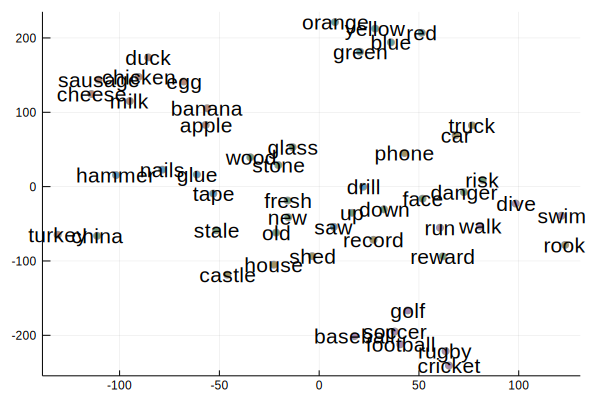
\includegraphics[width=\textwidth]{figs/chapterwordrepr/wordembvisual}
\end{figure}


Word embeddings are vector representations of words.
An dimensionality reduced scatter plot example of some word embeddings is shown in  \Cref{fig:wordvectors}.


\section{Representations for Language Modeling}

\aside[Probability writing convention]{We follow convention that capitalised $\n W_i$ is a random variable, and $\n w_i$ is a particular value which $\n W_i$ may take. The probability of it taking that value would normally be written $P(\n W_i{=}\n w_i)$.
We simply write $P(\n w_i)$ to mean the same thing.
This is a common abridged (abuse-of) notation.
The random variable in question is implicitly given by the name of its value.
}

The language modeling task is to predict the next word given the prior words \pcite{rosenfeld2000two}.
For example, if a sentence begins \natlang{For lunch I will have a hot}, then there is a high probability that the next word will be \natlang{dog} or \natlang{meal},
and lower probabilities of words such as \natlang{day} or \natlang{are}.
Mathematically it is formulated as: 
\begin{equation}\label{equ:langmodel}
	P(\n W_i{=}\n w_i \mid \n W_{i-1}{=}\n w_{i-1}, \ldots, \n W_1{=}\n w_1)
\end{equation}
or to use the compact notation 
\begin{equation}\label{equ:langmodelcompact}
P(\n w_i \mid \n w_{i-1}, \ldots, \n w_1)
\end{equation}
where $\n W_i$ is a random variable for the ith word, and $\n w_i$ is a value (a word) it could, (or does) take.
For example: 
\begin{equation*}
P(\natlang{dog} \mid \natlang{hot}, \natlang{a}, \natlang{want}, \natlang{I}, \natlang{lunch}, \natlang{For})
\end{equation*}
The task is to find the probabilities for the various words that $\n w_i$ could represent.

\aside[Google n-gram corpora]{Google has created a very large scale corpora of 1,2,3,4, and 5-grams from over $10^{12}$ words from the Google Books project. It has been made freely available at \url{https://books.google.com/ngrams/datasets} \parencite{lin2012syntactic}.
Large scale n-gram corpora are also used outside of statistical language modeling by corpus linguists investigating the use of language.
}

  
The classical approach is trigram statistical language modeling.
In this, the number of occurrences of word triples in a corpus is counted.
From this joint probability of triples, one can condition upon the first two words,
to get a conditional probability of the third.
This makes the Markov assumption that the next state depends only on the current state,
and that that state can be described by the previous two words.
Under this assumption \Cref{equ:langmodelcompact} becomes:
\begin{equation}\label{equ:trigramlangmodel}
P(\n w_i \mid \n w_{i-1}, \ldots, \n w_1) = P(\n w_i \mid \n w_{i-1}, \n w_{i-2})
\end{equation}
More generally, one can use an $n$-gram language model where for any value of $n$,
this is simply a matter of defining the Markov state to contain different numbers of words.

This Markov assumption is, of-course, an approximation.
In the previous example, a trigram language model finds $P(\n w_i \mid \natlang{hot}, \natlang{a})$.
It can be seen that the approximation has lost key information.
Based only on the previous 2 words the next word $\n w_i$ could now reasonably be \natlang{day}, but the sentence: \natlang{For lunch I will have a hot day} makes no sense.
However, the Markov assumption in using $n$-grams is required in order to make the problem tractable -- otherwise an unbounded amount of information would need to be stored. 

A key issue with n-gram language models is that there exists a data-sparsity problem which causes issues in training them.
Particularly for larger values of $n$.
Most combinations of words occur very rarely \pcite{ha2009extending}.
It is thus hard to estimate their occurrence probability.
Combinations of words that do not occur in the corpus are naturally given a probability of zero.
This is unlikely to be true though -- it is simply a matter of rare phrases never occurring in a finite corpus.
Several approaches have been taken to handle this.
The simplest is add-one smoothing which adds an extra ``fake'' observation to every combination of terms.
In common use are various back-off methods \pcite{katz1987estimation,kneser1995improved} which use the bigram probabilities to estimate the probabilities of unseen trigrams (and so forth for other n-grams.).
%
\aside{An extended look at classical techniques in statistical language modelling can be found in \textcite{DBLP:journals/corr/cs-CL-0108005}}
%
However, these methods are merely clever statistical tricks -- ways to reassign probability mass  to leave some left-over for unseen cases.
Back-off is smarter than add-one smoothing, as it portions the probability fairly based on the $(n{-}1)$-gram probability.
Better still would be a method which can learn to see the common-role of words \pcite{brown1992class}.
By looking at the fragment: \natlang{For lunch I want a hot}, any reader knows that the next word is most likely going to be a food.
We know this for the same reason we know the next word in \natlang{For elevenses  I had a cold \ldots} is also going to be a food.
Even though \natlang{elevenses} is a vary rare word, we know from the context that it is a meal (more on this later), and we know it shares other traits with meals, and similarly \natlang{have} / \natlang{had}, and \natlang{hot} / \natlang{cold}.
These traits influence the words that can occur after them.
Hard-clustering words into groups is nontrivial, particularly given words having multiple meanings, and subtle differences in use.
Thus the motivation is for a language modeling method which makes use of these shared properties of the words, but considers them in a flexible soft way.
This motivates the need for representations which hold such linguistic information.
Such representations must be discoverable from the corpus, as it is beyond reasonable to effectively hard-code suitable feature extractors.
This is exactly the kind of task which a neural network achieves implicitly in its internal representations.


\subsection{The Neural Probabilistic Language Model}\label{sec:the-neural-probabilistic-language-model}

\tcite{NPLM} present a method that uses a neural network to create a language model.
In doing so it implicitly learns the crucial traits of words, during training.
The core mechanism that allowed this was using an embedding or loop-up layer for the input.


\aside[Lookup word embeddings: Hashmap or Array?]{
	The question is purely one of implementation.
	For purposes of the theory, it does not matter if the implementation is using a String to Vector dictionary (e.g. a hashmap), or a 2D array from which a column is indexed-out (sliced-from) via an integer index representing the word.
	In the tokenization of the source text, it is common to transform all the words into integers, so as to save memory, especially if string interning is not in use.
	At that point it makes sense to work with an array.
	For our notational purposes in this book, we will treat the word $\n w_i$ as if it were an integer index, though thinking of it as a string index into a hashmap changes little in the logic.
}


\subsubsection{Simplified Model considered with Input Embeddings}
To understand the neural probabilistic language model, let's first consider a simplified neural trigram language model.
This model is a simplification of the model introduced by \textcite{NPLM}.
It follows the same principles, and highlights the most important idea in neural language representations.
This is that of training a vector representation of a word using a lookup table to map a discrete scalar word to a continuous-space vector which  becomes the first layer of the network.



The  neural trigram probabilistic network is defined by:
%
\begin{multline}
P(\n w_i \mid \n w_{i-1}, \n w_{i-2}) = \\
\softmax\left(V\varphi\left(U\left[\i C_{\n w_{i-1}}; \i C_{\n w_{i-2}}\right] + \v b \right) + \v k \right)
\end{multline}
%
where $U,\: V,\: \v b,\: \v k$ are the weight matrices and biases of the network.
The matrix $C$ defines the embedding table, 
from which the word embeddings, $\i C_{\n w_{i-1}}$ and $\i C_{\n w_{i-2}}$, representing the previous two words ($\n w_{i-1}$ and $\n w_{i-2}$) are retrieved.
The network is shown in \Cref{fig:trigram-neural-language-model}

\begin{figure}
	\caption{The Neural Trigram Language Model}
	\label{fig:trigram-neural-language-model} 
	\centering
	\documentclass{article}

\usepackage{tikz}
\usetikzlibrary{positioning, fit,  shapes.geometric}
\usepackage{ifthen}
\usepackage{etoolbox}

\tikzset{
	backgroundcolor/.style ={fill=white},
	every node/.append style={
		minimum height=7mm,
	},
	labe/.append style={
		%Blue,
		align = center,
		backgroundcolor,
		fill opacity=0.6,
		text opacity=1,
		font={\footnotesize\itshape}	
	},
	layer/.append style={
		draw,
		align = center,
		minimum height=7mm,
	},
	tight/.append style={
		inner sep=0.2mm,
	},
	lookupbox/.append style={
		draw=none,
		append after command={
		       	[shorten <= -0.5\pgflinewidth]
		       	([shift={(-1.5\pgflinewidth,-0.5\pgflinewidth)}]\tikzlastnode.north east)
		       	edge([shift={( 0.5\pgflinewidth,-0.5\pgflinewidth)}]\tikzlastnode.north west) 
		       	([shift={( 0.5\pgflinewidth,-0.5\pgflinewidth)}]\tikzlastnode.north west)
		       	edge([shift={( 0.5\pgflinewidth,-1.5\pgflinewidth)}]\tikzlastnode.south west)            
		       	([shift={( -1.5\pgflinewidth,+0.5\pgflinewidth)}]\tikzlastnode.south east)
		       	edge([shift={(-1.5\pgflinewidth,-0.5\pgflinewidth)}]\tikzlastnode.north east)
		},
		inner sep=0.7mm,
		outer sep=0mm,
		minimum width=25mm
	}
}

\begin{document}

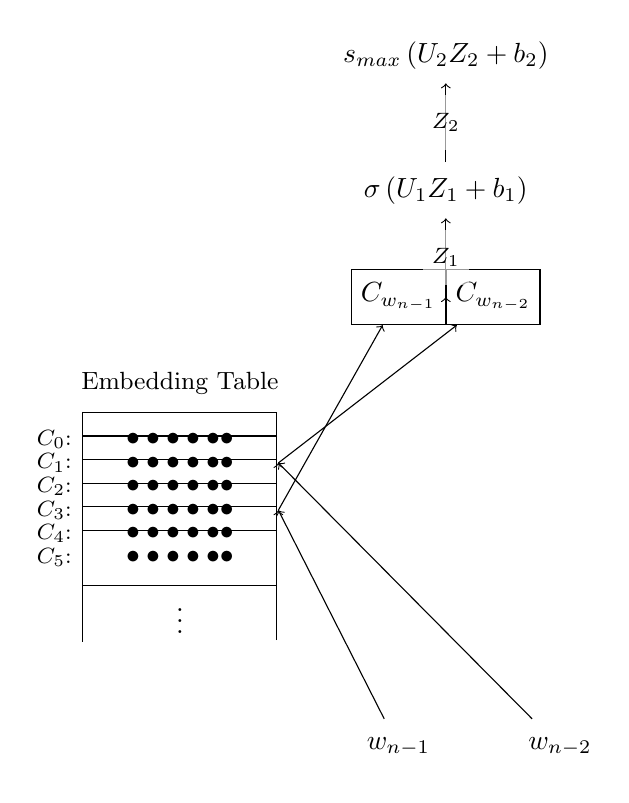
\begin{tikzpicture}[]


\node(w1) {$w_{n-1}$};
\node(w2)[right = of w1] {$w_{n-2}$};


\node(Cn)[lookupbox, above left=of w1] {$\vdots$};
\def\tblmax{6}
\foreach \ii in {1,...,\tblmax} {
	\pgfmathsetmacro\pos{(\ii - 1) * 3 };
	\pgfmathtruncatemacro\jj{(\tblmax -\ii)};
	
	\node(C\ii)[lookupbox, above = \pos mm of Cn]{$\bullet\bullet\bullet\bullet\bullet\bullet$};
	\node(Clbl\ii)[left = 0mm of C\ii]{\footnotesize $C_\jj$:};
};
\node(C)[above = 0mm of C\tblmax] {\small Embedding Table};



\node(concat1)[layer, above = 5 of w1]{$C_{w_{n-1}}$};
\node(concat2)[layer, right = 0 of concat1]{$C_{w_{n-2}}$};

\draw[->] (w1) edge (C3.east);
\draw[->]  (C3.east) edge (concat1);
\draw[->] (w2) edge (C5.east);
\draw[->]  (C5.east) edge (concat2);

\node(L1)[above = of concat1.east]{$\sigma\left(U_1Z_1 + b_1\right)$};
\draw[->]  (concat1.east) edge node[labe]{$Z_1$} (L1);

\node(L2)[above = of L1]{$s_{max}\left(U_2 Z_2 + b_2\right)$};
\draw[->]  (L1) edge node[labe]{$Z_2$} (L2);

\end{tikzpicture}

\end{document} 
\end{figure}

\aside[$\i C_{\n w_i}$ not $\i C_i$]{
Note that here we use the word $\n w_i$ as the index to lookup the word embeddings.
$i$ is the index of the word index in the corpus.
That is to say that if the $i$th word, and the $j$th word are the same: i.e $\n w_i = \n w_j$, then they will index out the same vector from $C$.
$\n w_i = \n w_j \implies \i C_{\n w_i} =  \i C_{\n w_j}$.
}


\aside[One-hot product or Indexed-lookup]{
	In some works you may see the process of retrieving the word vector from a matrix of word vectors described as a one-hot multiplication.
	For a word represented by the index $w$,
	where $\nv e_w$ the one-hot vector with a 1 in the $w$th position,
	and for $C$, the table of word embeddings,
	one can write  $C\,\nv e_w$ to find the embedding for $w$.
	We will write $\i C_w$ and refer to this as looking up the word vector from the $w$th column.
	Of-course $\i C_w=C\,\nv e_w$, however in practical implementation the performance ramifications are huge.
	Matrix column indexing is effectively an $O(1)$ operation (in a column major languages),
	whereas a dense matrix-vector product is $O(n^2)$.
	%
	The one-hot product can be used in a pinch to support using embeddings in neural network toolkits that do not support lookup/embedding layers.
	However, we strongly suggest that if your toolkit does not support lookup/embedding layers then it is unsuitable for use in NLP applications.
	%
	Some tool-kits, e.g. Flux.jl (\url{https://github.com/FluxML/Flux.jl}),
	explicitly handle sparse one-hot types, and automatically make this transformation.
	In that case, it is outright equivalent.
}

In the neural trigram language model, each of the previous two words is used to look-up a vector from the embedding matrix.
These are then concatenated to give a dense, continuous-space input to the above hidden layer.
The output layer is a softmax layer, it gives the probabilities for each word in the vocabulary,
such that $\i \hat{y}_{\n w_i} = P(\n w_i \mid \n w_{i-1}, \n w_{i-2})$.
Thus producing a useful language model.

The word embeddings are trained, just like any other parameter of the network (i.e. the other weights and biases) via gradient descent.
An effect of this is that the embeddings of words which predict the same future word will be adjusted to be nearer to each other in the vector space.
The hidden layer learns to associate information with regions of the embedding space, as the whole network (and every layer) is a continuous function.
This effectively allows for information sharing between words.
If two word's vectors are close together because they mostly predict the same future words, then that area of the embedding space is associated with predicting those words.
If words $a$ and $b$  often occur as the word prior to some similar set of words ($w,x,y,\ldots$) in the training set
and word $b$ also often occurs in the training set before word $z$, but (by chance) $a$ never does,
then this neural language model will predict that $z$ is likely to occur after $a$.
Where-as an n-gram language model would not.
This is because $a$ and $b$ have similar embeddings, due to predicting a similar set of words.
The model has learnt common features about these words implicitly from how they are used, and can use those to make better predictions.
These features are stored in the embeddings which are looked up during the input.

\subsubsection{Simplified Model considered with input and output embeddings}
We can actually reinterpret the softmax output layer as also having embeddings.
An alternative but equivalent diagram is shown in \Cref{fig:trigram-adv-neural-language-model}.

\begin{figure}
	\caption{Neural Trigram Language Model as considered with output embeddings. This is mathematically identical to \Cref{fig:trigram-neural-language-model}}
	\label{fig:trigram-adv-neural-language-model}
	\centering
	\documentclass{standalone}

\usepackage{tikz}
\usetikzlibrary{positioning, fit,  shapes.geometric}
\usepackage{ifthen}
\usepackage{etoolbox}

\tikzset{
	backgroundcolor/.style ={fill=white},
	every node/.append style={
		minimum height=7mm,
	},
	labe/.append style={
		%Blue,
		align = center,
		backgroundcolor,
		fill opacity=0.6,
		text opacity=1,
		font={\footnotesize\itshape}	
	},
	layer/.append style={
		draw,
		align = center,
		minimum height=7mm,
	},
	tight/.append style={
		inner sep=0.2mm,
	},
	lookupbox/.append style={
		draw=none,
		append after command={
		       	[shorten <= -0.5\pgflinewidth]
		       	([shift={(-1.5\pgflinewidth,-0.5\pgflinewidth)}]\tikzlastnode.north east)
		       	edge([shift={( 0.5\pgflinewidth,-0.5\pgflinewidth)}]\tikzlastnode.north west) 
		       	([shift={( 0.5\pgflinewidth,-0.5\pgflinewidth)}]\tikzlastnode.north west)
		       	edge([shift={( 0.5\pgflinewidth,-1.5\pgflinewidth)}]\tikzlastnode.south west)            
		       	([shift={( -1.5\pgflinewidth,+0.5\pgflinewidth)}]\tikzlastnode.south east)
		       	edge([shift={(-1.5\pgflinewidth,-0.5\pgflinewidth)}]\tikzlastnode.north east)
		},
		inner sep=0.7mm,
		outer sep=0mm,
		minimum width=25mm
	}
}
\usepackage{amsmath, amssymb, stmaryrd, mathtools}
\DeclareMathOperator*{\argmin}{argmin}
\DeclareMathOperator*{\argmax}{argmax}

\usepackage{xparse,xstring,etoolbox}
% crossref this against notation section
\newcommand{\vv}[1]{\tilde{#1}} % vector
\newcommand{\seq}[1]{\mathcal{#1}} % sequence
\newcommand{\set}[1]{\mathbb{#1}} % set

%%%%%%%%%
% Indexing/sequence indexing
\newcommand{\seqind}[2]{#1^{#2}} % seqence index
\newcommand{\ind}[2]{#1_{#2}} % indexed
\newcommand{\disamb}[2]{#1^{\mathrm{#2}}} %disambiguated

%% Smart indexing and naming
\newcommand{\ifupper}[3]{
    \normalexpandarg
	\exploregroups
	\StrCount{ABCDEFGHIJKLMNOPQRSTUVWXYZ}{#1}[\uppercount]
	\ifnumgreater{\uppercount}{0}{#2}{#3}
}

%smart index
\DeclareDocumentCommand{\ii}{u{_} m}{
	\ifupper{#1}%
	{% just a single uppercase character, i.e. a matrix
		  %make sure the index is the right length
		\StrCount{#2}{,}[\indcount]
		\ifnumgreater{\indcount}{0}
		{ % Got multiple indexes so all good
		 	\ind{#1}{#2}
		}
		{ % Only 1 index so grab the column
		 	\ind{#1}{{:,#2}}
		}
	}%
	{% Not just a single upper case character
		\ind{#1}{#2}
	}
}

\DeclareDocumentCommand{\nn}{u{_} m}{
	\seqind{#1}{#2}
}

\DeclareDocumentCommand{\dd}{u{_} m}{
	\disamb{#1}{#2}
}

% Index of a vector
\DeclareDocumentCommand{\iv}{u{_} m}{\ii{\vv #1}_{#2}}
\DeclareDocumentCommand{\dv}{u{_} m}{\dd{\vv #1}_{#2}}
\DeclareDocumentCommand{\nv}{u{_} m}{\nn{\vv #1}_{#2}}

%exp
\let\oldexp\exp
\renewcommand{\exp}[1]{\oldexp \left( #1 \right)}
\newcommand{\exptwo}[1]{\oldexp_2 \left( #1 \right)}

\newcommand{\softmax}{\mathrm{smax}}

\DeclareMathOperator*{\expectedop}{\mathbb{E}}
\DeclareDocumentCommand{\expected}{u{_} m}{
	\expectedop\limits_{\mathrlap{#2}}
}
\usetikzlibrary{calc}
\begin{document}

\begin{tikzpicture}[]


\node(w1) {$\n w_{i-1}$};
\node(w2)[right = of w1] {$\n w_{i-2}$};


\node(Cn)[lookupbox, above left=of w1] {$\vdots$};
\def\tblmax{6}
\foreach \ii in {1,...,\tblmax} {
	\pgfmathsetmacro\pos{(\ii - 1) * 3 };
	\pgfmathtruncatemacro\jj{(\tblmax -\ii)};
	
	\node(C\ii)[lookupbox, above = \pos mm of Cn]{$\bullet\bullet\bullet\bullet\bullet\bullet$};
	\node(Clbl\ii)[left = 0mm of C\ii]{\footnotesize $\i C_\jj$:};
};
\node(C)[above = 0mm of C\tblmax.north, text width=40] {\small \textsc{Input \\Embedding Table}};


\node(concat1)[layer, above = 5 of w1]{$\i C_{\n w_{i-1}}$};
\node(concat2)[layer, right = 0 of concat1]{$\i C_{\n w_{i-2}}$};

\draw[->] (w1) edge (C3.east);
\draw[->]  (C3.east) edge (concat1.south);
\draw[->] (w2) edge (C5.east);
\draw[->]  (C5.east) edge (concat2.south);

\node(L1)[layer, above = of concat1.north east]{$\varphi\left(U\,\dv z_{embs} + \v b\right)$};
\draw[->]  (concat1.north east) -- node[labe]{$\dv z_{embs}$} (L1);

$\frac{\exp{\i V_{\n w_i,:} \dv z_{hid} + \iv k_{\n w_i,:}}}%
{\sum_{\forall j} \exp{\i V_{j,:} \dv z_{hid} + \iv k_j}}$
};
\draw[->]  (L1) edge node[labe]{$\dv z_{hid}$} (L2);


\node(out)[above = of L2]{$P(\n w_i \mid \n w_{i-1}, \n w_{i-2})$};
\draw[->] (L2) edge (out);

\node(Vn)[lookupbox, above = 5 of Cn] {$\vdots$};
\def\tblmax{6}
\foreach \ii in {1,...,\tblmax} {
	\pgfmathsetmacro\pos{(\ii - 1) * 3 };
	\pgfmathtruncatemacro\jj{(\tblmax -\ii)};
	
	\node(V\ii)[lookupbox, above = \pos mm of Vn]{$\bullet\bullet\bullet\bullet\bullet\bullet$};
	\node(Vlbl\ii)[left = 0mm of V\ii]{\footnotesize $\i V_{\jj,:}$:};
	
	\pgfmathsetmacro\ang{(\ii * -2 + -180+20 };
	\draw[->] (V\ii.east) -- (L2.\ang);
};
\draw[->] (Vn.east) -- (L2.south west);
\node(C)[above = 0mm of V\tblmax.north, text width=40] {\small \textsc{Output \\Embedding Table}};




\draw[->] (out.204) -- (V6.east);
\draw[->] (V6.east)-- (L2.120);

\end{tikzpicture}

\end{document} 
\end{figure}

\aside[Consider, that the matrix product of a row vector with a column vector is the dot product]{
	$\i V_{w_{i},:} \dv z_{hid}$ can be seen as computing the dot product
	between the output embedding for $w_{i}$ and the hidden layer representation
	of the prior words/context ($\n w_{i-1}$ and $\n w_{i-2}$ in this case) in the form of $\dv z_{hid}$.
	This leads to an alternate interpretation of the whole process as minimising the dot-product distance between the output embedding and the context representation
	This is particularly relevant for the skip-gram model discussed in \Cref{sec:skip-gram} (with just one input word and no hidden layer).	
}
The final layer of the neural trigram language model can be rewritten per each index corresponding to a possible next word ($\n w_i$):
\begin{equation}
\i {\softmax(V \dv z_{hid}+ \v k)}_{\n w_i} = \dfrac{\exp{\i V_{\n w_i,:} \dv z_{hid}+\iv k_{\n w_i}}}{\sum_{\forall j}\exp{\i V_{j,:} \dv z_{hid}+\iv k_{j}}}
\end{equation} 


In this formulation, we have $\i V_{w_{i},:}$ as the output embedding for $\n w_{i}$.
As we considered  $\i C_{w_{i}}$ as its input embedding.


\subsubsection{Bayes-like Reformulation}
When we consider the model with output embeddings, 
it is natural to also consider it under the light of the Bayes-like reformulation from \Cref{sec:softmax-and-bayes-theorem}:
\begin{multline}
P(Y{=}i\mid Z{=}\v z)=\frac{R(Z{=}\v z\mid Y{=}i)\,R(Y{=}i)}{\sum_{\forall j}R(Z{=}\v z\mid Y{=}j)\,R(Y{=}j)}
\end{multline}
which in this case is:
\begin{multline}
P(\n w_{i}\mid \n w_{i-1},\n w_{i-2})=\\
\frac{R(Z{=}\dv z_{hid} \mid \n W_{i}{=} \n w_{i})\,R(\n W_{i}{=}\n w_{i})}{
	\sum_{\forall v \in \set V}R(Z=\dv z_{hid}\mid \n W_{i} {=} v)\,R(\n W_{i}{=}v)
}
\end{multline}
where $\sum_{\forall v \in \set V}$ is summing over every possible word $v$ from the vocabulary $\set V$,
which does include the case $v=\n w_i$.

Notice the term:
\begin{align}
\frac{R(\n W_{i}{=}\n w_{i})}{\sum_{\forall v \in \set V} R(\n W_{i}{=}v)} 
&= \frac{\exp{\iv k_{\n w_i}}}{\sum_{\forall v \in \set V} \exp{\iv k_{v}}}\\
&= \frac{1}{\sum_{\forall v \in \set V} \exp{\iv k_{v} - \iv k_{\n w_i}}}
\end{align}


The term $R(\n W_{i}{=}\n w_i)=\exp{\iv k_{\n w_i}}$ is linked to the unigram word probabilities: $P(Y=y)$.
If $\mathbb{E}(R(Z\mid W_{i})=1$ then the optimal value for $\v k$ would be given by the log unigram probabilities: $k_{\n w_i}=\log P(\n W_{i}{=} \n w_{i})$.
This condition is equivalent to if $\mathbb{E}(V\dv z_{hid})=0$.
Given that  $V$ is normally\footnote{no pun intended} initialized as a zero mean Gaussian, this condition is at least initially true.
This suggests, interestingly, that we can predetermine good initial values for the output bias $\v k$ using the log of the unigram probabilities.
In practice this is not required, as it is learnt rapidly by the network during training.


\subsubsection{The Neural Probabilistic Language Model}
\tcite{NPLM} derived a more advanced version of the neural language model discussed above.
Rather than being a trigram language model, it is an $n$-gram language model, where $n$ is a hyper-parameter of the model.
The knowledge sharing allows the data-sparsity issues to be ameliorated, thus allowing for a larger $n$ than in traditional n-gram language models.
%
\aside[Input vocabulary and output vocabulary do not have to be the same]{\textcite{schwenk2004efficient} suggests using only a subset of the vocabulary as options for the output, while allowing the full vocabulary in the input space -- with a fall-back to classical language models for the missed words.
This decreases the size of the softmax output layer, which substantially decreases the time taken to train or evaluate the network.
As a speed-up technique this is now eclipsed by hierarchical softmax and negative sampling discussed in \Cref{sec:hierachical-softmax-and-negative-sampling}.
The notion of a different input and output vocabulary though remains important for word-sense embeddings as will be discussed in \Cref{sec:word-sense-representations}.
}
%
\textcite{NPLM} investigated values for 2, 4 and 5 prior words (i.e. a trigram, 5-gram and 6-gram model).
The network used in their work was marginally more complex than the trigram neural language model.
As shown in \Cref{fig:neural-language-model}, it features a layer-bypass connection.
For $n$ prior words, the model is described by:
\begin{align}
P(\n w_i & \mid \n w_{i-1}, \ldots, \n w_{i-n}) = \softmax( \nonumber
\\  & + V \: \varphi\left( \d U_{hid} \left[\i C_{\n w_{i-1}};\ldots; \i C_{\n w_{i-n}} \right] + \v b\right) \nonumber
\\  & + \d U_{bypass} \left[ \i C_{\n w_{i-1}};\ldots; \i C_{\n w_{i-n}}\right] \nonumber
\\  & + \v k 
\i{)}_{\n w_i} % hack
\end{align}


The layer-bypass is a connivance to aid in the learning.
It allows the input to directly affect the output without being mediated by the shared hidden layer.
This layer-bypass is an unusual feature, not present in future works deriving from this, such as \tcite{schwenk2004efficient}.
Though in general it is not an unheard of technique in neural network machine learning.


This is the network which begins the notions of using neural networks with vector representations of words.
Bengio et al. focused on the use of the of sliding window of previous words -- much like the traditional n-grams.
At each time-step the window is advanced forward and the next is word predicted based on the shifted context of prior words.
This is of-course exactly identical to extracting all n-grams from the corpus and using those as the training data.
They very briefly mention that an RNN could be used in its place.

\begin{figure}
	\caption{Neural Probabilistic Language Model}
	\label{fig:neural-language-model}
	\centering
	\documentclass{article}

\usepackage{tikz}
\usetikzlibrary{positioning, fit,  shapes.geometric}
\usepackage{ifthen}
\usepackage{etoolbox}

\tikzset{
	backgroundcolor/.style ={fill=white},
	every node/.append style={
		minimum height=7mm,
	},
	labe/.append style={
		%Blue,
		align = center,
		backgroundcolor,
		fill opacity=0.6,
		text opacity=1,
		font={\footnotesize\itshape}	
	},
	layer/.append style={
		draw,
		align = center,
		minimum height=7mm,
	},
	tight/.append style={
		inner sep=0.2mm,
	},
	lookupbox/.append style={
		draw=none,
		append after command={
		       	[shorten <= -0.5\pgflinewidth]
		       	([shift={(-1.5\pgflinewidth,-0.5\pgflinewidth)}]\tikzlastnode.north east)
		       	edge([shift={( 0.5\pgflinewidth,-0.5\pgflinewidth)}]\tikzlastnode.north west) 
		       	([shift={( 0.5\pgflinewidth,-0.5\pgflinewidth)}]\tikzlastnode.north west)
		       	edge([shift={( 0.5\pgflinewidth,-1.5\pgflinewidth)}]\tikzlastnode.south west)            
		       	([shift={( -1.5\pgflinewidth,+0.5\pgflinewidth)}]\tikzlastnode.south east)
		       	edge([shift={(-1.5\pgflinewidth,-0.5\pgflinewidth)}]\tikzlastnode.north east)
		},
		inner sep=0.7mm,
		outer sep=0mm,
		minimum width=25mm
	}
}

\begin{document}

\begin{tikzpicture}[]


\node(w1) {$\n w_{i-1}$};
\node(w2)[right = 0mm  of w1] {$\n w_{i-2}$};
\node(w3)[right = 0mm of w2] {$\ldots$};
\node(w4)[right = 0mm of w3] {$\n w_{i-n}$};


\node(Cn)[lookupbox, above left=of w1] {$\vdots$};
\def\tblmax{6}
\foreach \ii in {1,...,\tblmax} {
	\pgfmathsetmacro\pos{(\ii - 1) * 3 };
	\pgfmathtruncatemacro\jj{(\tblmax -\ii)};
	
	\node(C\ii)[lookupbox, above = \pos mm of Cn]{$\bullet\bullet\bullet\bullet\bullet\bullet$};
	\node(Clbl\ii)[left = 0mm of C\ii]{\footnotesize $\i C_\jj$:};
};
\node(C)[above = 0mm of C\tblmax] {\small \textsc{Embedding Table}};


\node(concat1)[layer, above = 5 of w1]{$\i C_{\n w_{i-1}}$};
\node(concat2)[layer, right = 0 of concat1]{$\i C_{\n w_{i-2}}$};
\node(concat3)[layer, right = 0 of concat2]{$\quad\ldots\quad$};
\node(concat4)[layer, right = 0 of concat3]{$\i C_{\n w_{i-n}}$};
 
\draw[->] (w1) edge (C3.east);
\draw[->]  (C3.east) edge (concat1.south);
\draw[->] (w2) edge (C5.east);
\draw[->]  (C5.east) edge (concat2.south);
\draw[->] (w4) edge (C5.east);
\draw[->]  (C5.east) edge (concat4.south);

\node(L1)[layer, above = of concat2.north east]{$\varphi\left(\d U_{hid}\dv z_{embs} + \v b\right)$};
\draw[->]  (concat2.north east) -- node[labe]{$\dv z_{embs}$} (L1);


\node(L2)[layer, above = of L1]{$s_{max}\left(V \dv z_{hid} +\d U_{bypass} \dv z_{embs}+ \v k\right)$};
\draw[->]  (L1) edge node[labe]{$\dv z_{hid}$} (L2); 
\draw[->, bend right] (concat2.north east)  to[bend right=45, min distance=25 mm] (L2);


\node(out)[above = of L2]{$P(\n w_i \mid \n w_{i-1}, \n w_{i-2}, \ldots, \n w_{i-n})$};
\draw[->] (L2) edge (out);


\end{tikzpicture}

\end{document} 
\end{figure}


\subsection{RNN Language Models}
\begin{figure}
	\caption{RNN Language Model. The RU equation shown is the basic RU used in \textcite{mikolov2010recurrent}.
	It can be substituted for a LSTM RU or an GRU as was done in \textcite{sundermeyer2012lstm,jozefowicz2015empirical}, with appropriate changes.
	}
	\label{fig:neural-language-model}
	\centering
	\resizebox{\textwidth}{!}{\documentclass{article}

\usepackage{tikz}
\usetikzlibrary{positioning, fit,  shapes.geometric}
\usepackage{ifthen}
\usepackage{etoolbox}

\tikzset{
	backgroundcolor/.style ={fill=white},
	every node/.append style={
		minimum height=7mm,
	},
	labe/.append style={
		%Blue,
		align = center,
		backgroundcolor,
		fill opacity=0.6,
		text opacity=1,
		font={\footnotesize\itshape}	
	},
	layer/.append style={
		draw,
		align = center,
		minimum height=7mm,
	},
	tight/.append style={
		inner sep=0.2mm,
	},
	lookupbox/.append style={
		draw=none,
		append after command={
		       	[shorten <= -0.5\pgflinewidth]
		       	([shift={(-1.5\pgflinewidth,-0.5\pgflinewidth)}]\tikzlastnode.north east)
		       	edge([shift={( 0.5\pgflinewidth,-0.5\pgflinewidth)}]\tikzlastnode.north west) 
		       	([shift={( 0.5\pgflinewidth,-0.5\pgflinewidth)}]\tikzlastnode.north west)
		       	edge([shift={( 0.5\pgflinewidth,-1.5\pgflinewidth)}]\tikzlastnode.south west)            
		       	([shift={( -1.5\pgflinewidth,+0.5\pgflinewidth)}]\tikzlastnode.south east)
		       	edge([shift={(-1.5\pgflinewidth,-0.5\pgflinewidth)}]\tikzlastnode.north east)
		},
		inner sep=0.7mm,
		outer sep=0mm,
		minimum width=25mm
	}
}

\begin{document}

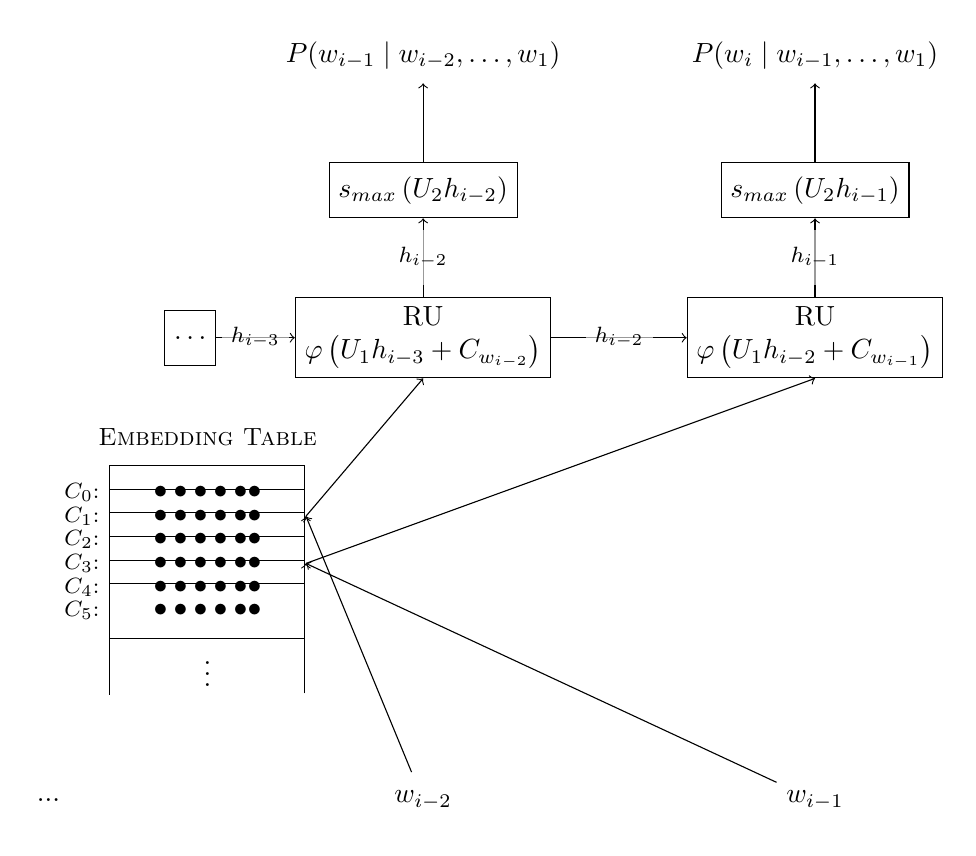
\begin{tikzpicture}[]

\newcommand{\hsep}{4}
\newcommand{\vtablesep}{5}

\node(w1) {$w_{i-1}$};
\node(w2)[left = \hsep of w1] {$w_{i-2}$};
\node(w3)[left = \hsep of w2] {$...$};


\node(Cn)[lookupbox, above left=of w2] {$\vdots$};
\def\tblmax{6}
\foreach \ii in {1,...,\tblmax} {
	\pgfmathsetmacro\pos{(\ii - 1) * 3 };
	\pgfmathtruncatemacro\jj{(\tblmax -\ii)};
	
	\node(C\ii)[lookupbox, above = \pos mm of Cn]{$\bullet\bullet\bullet\bullet\bullet\bullet$};
	\node(Clbl\ii)[left = 0mm of C\ii]{\footnotesize $C_\jj$:};
};
\node(C)[above = 0mm of C\tblmax] {\small \textsc{Embedding Table}};

\node(L11)[layer, above = \vtablesep of w1]{RU\\$\varphi\left( U_1h_{i-2}  +  C_{w_{i-1}}\right)$};
\node(L21)[layer, above = of L11]{$s_{max}\left(U_2 h_{i-1}\right)$};
\draw[->]  (L11) edge node[labe]{$h_{i-1}$} (L21);
\node(out1)[above = of L21]{$P(w_i \mid w_{i-1}, \ldots,  w_1)$};
\draw[->] (L21) edge (out1);

\node(L12)[layer, above = \vtablesep of w2]{RU\\$\varphi\left( U_1h_{i-3}  +  C_{w_{i-2}}\right)$};
\node(L22)[layer, above = of L12]{$s_{max}\left(U_2 h_{i-2} \right)$};
\draw[->]  (L12) edge node[labe]{$h_{i-2}$} (L22);
\node(out2)[above = of L22]{$P(w_{i-1} \mid w_{i-2}, \ldots,  w_1)$};
\draw[->] (L22) edge (out2);
\draw[->]  (L12) edge node[labe]{$h_{i-2}$} (L11);

\node(L13)[layer, left = of L12] {$\ldots$};
\draw[->]  (L13) edge node[labe]{$h_{i-3}$} (L12);


\draw[->] (w1) edge (C3.east);
\draw[->]  (C3.east) edge (L11.south);
\draw[->] (w2) edge (C5.east);
\draw[->]  (C5.east) edge (L12.south);


\end{tikzpicture}

\end{document}}
\end{figure}


In \tcite{mikolov2010recurrent} an RNN is used for language modelling.
Using the terminology of \Cref{sec:rnn}, this is an encoder RNN, made using Basic Recurrent Units.
Using an RNN eliminates the Markov assumption of a finite window of prior words forming the state.
Instead, the state is learned, and stored in the state component of the RUs. 

\aside[No Bias?]{It should be noticed that \Cref{equ:rnnlm1,equ:rnnlm2} are missing the bias terms.
	This is not commented on in \textcite{mikolov2010recurrent}.
	But in the corresponding chapter of Mikolov's thesis \parencite{mikolov2012thesis},
	it is explicitly noted that biases were not used in the network as it was not found that they gave a significant improvement to the result.
	This is perhaps surprising, particularly in the output softmax layer given the very unbalanced class (unigram) frequencies.
	
	In the papers for several of Mikolov's other works, including those for skip-gram and CBOW discussed in \Cref{sec:acausal-language-modeling}, the bias terms are also excluded.
	We have matched those equations here.  
	We do note though, that it is likely that many publicly available implementations of these algorithms would include the bias term:
	due either to a less close reading of the papers,
	or to the assumption that the equations are given in \emph{design matrix} form: where the bias is not treated as a separate term to the weights, and the input is padded with an extra 1.
	We do not think this is at all problematic.
	
	We discuss this further for the case of hierarchical softmax in \Cref{sec:hierarchical-softmax}, where the level is a proxy for the unigram frequency -- and thus for the bias.
}

This state $\iv h_{i}$ being the hidden state  (and output as this is a basic RU) from the $i$ time-step.
The $i$th time-step takes as its input the $i$th word.
As usual this hidden layer was an input to the hidden-layer at the next time-step, as well as to the output softmax.
%

%
\begin{align}
	\nv h_{i} &= \varphi\left( U\nv h_{i-1} + \i C_{w_{i-1}} \right) \label{equ:rnnlm1} \\
	P(\n w_i \mid \n w_{i-1}, \ldots \n w_{1}) &= \i {\softmax\left(V \nv h_{i-1} \right)}_{\n w_i} \label{equ:rnnlm2}
\end{align}


Rather than using a basic RU, a more advanced RNN such as a LSTM or GRU-based network can be used.
This was done by \tcite{sundermeyer2012lstm} and \tcite{jozefowicz2015empirical},
both of whom found that the more advanced networks gave significantly better results.

\section{Acausal Language Modeling}\label{sec:acausal-language-modeling}
The step beyond a normal language model,
which uses the prior words to predict the next word, is what we will term acausal language modelling.
Here we use the word acausal in the signal processing sense.
It is also sometimes called contextual language modelling, as the whole context is used, not just the prior context.
The task here is to predict a missing word, using the words that precede it, as well as the words that come after it.

As it is acausal it cannot be implemented in a real-time system, and for many tasks this renders it less, directly, useful than a normal language model. 
However, it is very useful as a task to learn a good representation for words.


\aside[Are CBOW \& Skip-Gram Neural Networks?]{It is sometimes asserted that these models are not in-fact neural networks at all.
This assertion is often based on their lack of a traditional hidden-layer, and similarities in form to several other mathematical models (discussed in \Cref{sec:co-location-factorisation}).
This distinction is purely academic though.
Any toolkit that can handle the prior discussed neural network models can be used to implement CBOW and Skip-Gram, more simply than using a non-neural network focused optimiser.
 
It also should be noted that embedding lookup is functionally an unusual hidden layer -- this becomes obvious when considering the lookup as an one-hot product. 
Though it does lack a non-linear activation function.

}


The several of the works discussed in this section also feature hierarchical softmax and negative sampling methods as alternative output methods.
As these are complicated and easily misunderstood topics they are discussed in a more tutorial fashion in \Cref{sec:hierachical-softmax-and-negative-sampling}.
This section will focus just on the language model logic; and assume the output is a normal softmax layer.

\subsection{Continuous Bag of Words}\label{sec:cbow}
\begin{figure}
	\caption{CBOW Language Model}
	\label{fig:cbow}
	\centering
	\resizebox{\textwidth}{!}{\documentclass{standalone}

\usepackage{tikz}
\usetikzlibrary{positioning, fit,  shapes.geometric}
\usepackage{ifthen}
\usepackage{etoolbox}

\tikzset{
	backgroundcolor/.style ={fill=white},
	every node/.append style={
		minimum height=7mm,
	},
	labe/.append style={
		%Blue,
		align = center,
		backgroundcolor,
		fill opacity=0.6,
		text opacity=1,
		font={\footnotesize\itshape}	
	},
	layer/.append style={
		draw,
		align = center,
		minimum height=7mm,
	},
	tight/.append style={
		inner sep=0.2mm,
	},
	lookupbox/.append style={
		draw=none,
		append after command={
		       	[shorten <= -0.5\pgflinewidth]
		       	([shift={(-1.5\pgflinewidth,-0.5\pgflinewidth)}]\tikzlastnode.north east)
		       	edge([shift={( 0.5\pgflinewidth,-0.5\pgflinewidth)}]\tikzlastnode.north west) 
		       	([shift={( 0.5\pgflinewidth,-0.5\pgflinewidth)}]\tikzlastnode.north west)
		       	edge([shift={( 0.5\pgflinewidth,-1.5\pgflinewidth)}]\tikzlastnode.south west)            
		       	([shift={( -1.5\pgflinewidth,+0.5\pgflinewidth)}]\tikzlastnode.south east)
		       	edge([shift={(-1.5\pgflinewidth,-0.5\pgflinewidth)}]\tikzlastnode.north east)
		},
		inner sep=0.7mm,
		outer sep=0mm,
		minimum width=25mm
	}
}
\usetikzlibrary{calc}
\begin{document}

\begin{tikzpicture}[]


\node(wn1) at (0,0) {$\n w_{i-1}$};
\node(wp1) [right = 0mm  of wn1] {$\n w_{i+1}$};
\node(wn2)[left = 0mm of wn1] {$\ldots$};
\node(wp2)[right = 0mm of wp1] {$\ldots$};
\node(wn3)[left = 0mm of wn2] {$\n w_{i-\frac{n}{2}}$};
\node(wp3)[right = 0mm of wp2] {$\n w_{i+\frac{n}{2}}$};


\coordinate[above left=of w1, xshift=-2cm] (CC0) at (-2.5,1);
\embtable{C}{CC0}{Input Embedding Table}

%\def\tblmax{6}
%\foreach \ii in {1,...,\tblmax} {
%	\pgfmathsetmacro\pos{(\ii - 1) * 3 };
%	\pgfmathtruncatemacro\jj{(\tblmax -\ii)};
%	
%	\node(C\ii)[lookupbox, above = \pos mm of Cn]{$\bullet\bullet\bullet\bullet\bullet\bullet$};
%	\node(Clbl\ii)[left = 0mm of C\ii]{\footnotesize $\i C_\jj$:};
%};
%\node(C)[above = 0mm of C\tblmax.north, text width=40] {\small \textsc{Input \\Embedding Table}};




\node(L2)[layer, above = 8 of wn1]{
$\softmax \left(V \sum_{j=1}^{j=\frac{n}{2}} \left( \i C_{\n w_{i-j}}+\i C_{\n w_{i+j}} \right)\right)$
};


\path[->, draw] (wp1) to ({C}3.east) edge[->] (L2.290);
\draw[->] (wp2) to ({C}n.east) edge[->] (L2.310);
\draw[->] (wp3) to ({C}1.east) edge[->] (L2.300);
\draw[->] (wn1) to ({C}2.east) edge[->] (L2.346);
\draw[->] (wn2) to ({C}n.east) edge[->] (L2.347);
\draw[->] (wn3) to ({C}4.east) edge[->] (L2.345);




\node(out)[above = of L2]{$P(\n w_i \mid \n w_{i-\frac{n}{2}},..., \n w_{i-1}, \n w_{i+1},...,\n w_{i+\frac{n}{2}}))$};
\draw[->] (L2) edge (out);



\end{tikzpicture}

\end{document}}
\end{figure}

The continuous bag of words (CBOW) method was introduced by \tcite{mikolov2013efficient}.
In truth, this is not particularly similar to bag of words at all.
No more so than any other word representation that does not have regard for order of the context words (e.g. skip-gram, and GloVe).

The CBOW model takes as its input a context window surrounding a central skipped word, and tries to predict the word that it skipped over.
It is very similar to earlier discussed neural language models, except that the window is on both sides.
It also does not have any non-linearities;
and the only hidden layer is the embedding layer.

For a context window of width $n$ words -- i.e. $\frac{n}{2}$ words to either side, of the target word $\n w_i$,
the CBOW model is defined by:
\begin{align}
P(\n w_i & \mid \n w_{i-\frac{n}{2}},\ldots, \n w_{i-1}, \n w_{i+1},\ldots, \n w_{i+\frac{n}{2}})  \nonumber
\\  & = \i {\softmax \left(V \sum_{j=i+1}^{j=\frac{n}{2}} \left( \i C_{\n w_{i-j}}+\i C_{\n w_{i+j}} \right)\right)}_{\n w_i}
\end{align}
This is shown in diagrammatic form in \Cref{fig:cbow}.
By optimising across a training dataset, useful word embeddings are found,
just like in the normal language model approaches.


\subsection{Skip-gram}\label{sec:skip-gram}
\begin{figure}
	\caption{Skip-gram language Language Model. Note that the probability $P(\n w_j \mid \n w_i)$ is optimised during training for every $\n w_j$ in a window around the central word $\n w_i$.
	Note that the final layer in this diagram is just a softmax layer, written in in output embedding form.}
	\label{fig:skip-gram} 
	\centering
	%\resizebox{\textwidth}{!}{
		\documentclass{standalone}

\usepackage{tikz}
\usetikzlibrary{positioning, fit,  shapes.geometric}
\usepackage{ifthen}
\usepackage{etoolbox}

\tikzset{
	backgroundcolor/.style ={fill=white},
	every node/.append style={
		minimum height=7mm,
	},
	labe/.append style={
		%Blue,
		align = center,
		backgroundcolor,
		fill opacity=0.6,
		text opacity=1,
		font={\footnotesize\itshape}	
	},
	layer/.append style={
		draw,
		align = center,
		minimum height=7mm,
	},
	tight/.append style={
		inner sep=0.2mm,
	},
	lookupbox/.append style={
		draw=none,
		append after command={
		       	[shorten <= -0.5\pgflinewidth]
		       	([shift={(-1.5\pgflinewidth,-0.5\pgflinewidth)}]\tikzlastnode.north east)
		       	edge([shift={( 0.5\pgflinewidth,-0.5\pgflinewidth)}]\tikzlastnode.north west) 
		       	([shift={( 0.5\pgflinewidth,-0.5\pgflinewidth)}]\tikzlastnode.north west)
		       	edge([shift={( 0.5\pgflinewidth,-1.5\pgflinewidth)}]\tikzlastnode.south west)            
		       	([shift={( -1.5\pgflinewidth,+0.5\pgflinewidth)}]\tikzlastnode.south east)
		       	edge([shift={(-1.5\pgflinewidth,-0.5\pgflinewidth)}]\tikzlastnode.north east)
		},
		inner sep=0.7mm,
		outer sep=0mm,
		minimum width=25mm
	}
}
\usetikzlibrary{calc}
\begin{document}

\begin{tikzpicture}[]


\node(w1) at (0,0) {$w_{i}$};


\node(Cn)[lookupbox] at (-4,1) {$\vdots$};
\def\tblmax{6}
\foreach \ii in {1,...,\tblmax} {
	\pgfmathsetmacro\pos{(\ii - 1) * 3 };
	\pgfmathtruncatemacro\jj{(\tblmax -\ii)};
	
	\node(C\ii)[lookupbox, above = \pos mm of Cn]{$\bullet\bullet\bullet\bullet\bullet\bullet$};
	\node(Clbl\ii)[left = 0mm of C\ii]{\footnotesize $C_\jj$:};
};
\node(C)[above = 0mm of C\tblmax.north, text width=40] {\small \textsc{Input \\Embedding Table}};


\draw[->] (w1) edge (C3.east);


\node(L2)[layer, above = 8 of w1]{
$\frac{\exp\left(V^\prime_{w_j} C_{w_i} + b_j \right)}%
{\sum_{\forall k}exp\left(V^\prime_{k} C_{w_i} + b_k \right)}$
};
\draw[->]  (C3.east) edge node[labe]{$C_{w_i}$} (L2);


\node(out)[above = of L2]{$P(w_j \mid w_i)$};
\draw[->] (L2) edge (out);

\node(Vn)[lookupbox, above = 5 of Cn] {$\vdots$};
\def\tblmax{6}
\foreach \ii in {1,...,\tblmax} {
	\pgfmathsetmacro\pos{(\ii - 1) * 3 };
	\pgfmathtruncatemacro\jj{(\tblmax -\ii)};
	
	\node(V\ii)[lookupbox, above = \pos mm of Vn]{$\bullet\bullet\bullet\bullet\bullet\bullet$};
	\node(Vlbl\ii)[left = 0mm of V\ii]{\footnotesize $V_\jj^\prime$:};
	
	\pgfmathsetmacro\ang{(\ii * -2 + -180+20 };
	\draw[->] (V\ii.east) -- (L2.\ang);
};

\draw[->] (Vn.east) -- (L2.south west);
\node(C)[above = 0mm of V\tblmax.north, text width=40] {\small \textsc{Output \\Embedding Table}};


\draw[->] (out.204) -- (V6.east);
\draw[->] (V6.east)-- node[labe]{$V_{w_j}^\prime$} (L2.170);

\end{tikzpicture}

\end{document}
	%}
\end{figure}


\aside[Skip-gram naming]{In different publications this model may be called skipgram, skip-gram, skip-ngram, skip gram etc. Further, it may be called \texttt{word2vec} after the publicly released implementation of the algorithm. Though the \texttt{word2vec} software can also be used for CBOW, so sometimes it can refer to CBOW.}

The converse of CBOW is the skip-grams model \tcite{mikolov2013efficient}.
In this model, the central word is used to predict the words in the context.
%Each window of words in the training set defines a number of training cases equal to its width -- minus the central word being used to predict.

The model itself is single word input, and its output is a softmax for the probability of each word in the vocabulary occurring in the context of the input word.
This can be indexed to get the individual probability of a given word occurring as usual for a language model.
So for input word $\n w_i$ the probability of $\n w_j$ occurring in its context is given by:
\begin{equation}
P(\n w_j \mid \n w_i) = \i {\softmax \left( V\,\i C_{\n w_i}) \right)}_{\n w_j} \label{equ:skipgram}
\end{equation}


The goal, is to maximise the probabilities of all the observed outputs that actually \emph{do} occur in its context.
This is done, as in CBOW by defining a window for the context of a word in the training corpus, ($i-\frac{n}{2},\ldots,i-1, i+i,\ldots,i+\frac{n}{2}$).
It should be understood that while this is presented similarly to a classification task,
there is no expectation that the model will actually predict the correct result,
given that even during training there are multiple correct results.
It is a regression to an accurate estimate of the probabilities of co-occurrence
(this is true for probabilistic language models more generally, but is particularly obvious in the skip-gram case).


Note that in skip-gram, like CBOW, the only hidden layer is the embedding layer.
Rewriting \Cref{equ:skipgram} in output embedding form:

\begin{align}
P(\n w_j \mid \n w_i) & = \i {\softmax \left(V\,\i C_{\n w_i}\right)}_{\n w_j} \\
P(\n w_j \mid \n w_i) & = \frac{\exp{\i V_{\n w_j,:} \i C_{\n w_i}}}{\sum_{\forall v \in \set V} \exp{\i V_{v,:}\i C_{v}}} \label{equ:skipgram-output}
\end{align}

The key term here is the product $\i V_{\n w_j,:}\,\i C_{\n w_i}$.
The remainder of \Cref{equ:skipgram-output}  is to normalise this into a probability.
Maximising the probability $P(\n w_j \mid \n w_i)$ is equivalent to maximising the dot produce between $\i V_{\n w_j,:}$, the output embedding for $\n w_j$ and  $\i C_{\n w_i}$ the input embedding for $\n w_i$.
This is to say that the skip-gram probability is maximised when the angular difference between the input embedding for a word, and the output embeddings for its co-occurring words is minimised.
The dot-product is a measure of vector similarity -- closely related ot the cosine similarity.

Skip-gram is much more commonly used than CBOW.


\subsection{Analogy Tasks}
\aside[Analogy Tasks uncover prejudice in corpora]{\textcite{bolukbasi2016man} and \textcite{Caliskan183} use analogy tasks, and related variant formulations to find troubling associations between words, such as Bolukbasi et. al's titular \natlang{Man} is to \natlang{Computer Programmer}, as \natlang{Woman} is to \natlang{Homemaker}. Finding these relationships in the embedding space, indicated that they are present in the training corpus, which in turn shows their prevalence  in society at large.
It has been observed that machine learning can be a very good mirror upon society.
}



\asidefig[\label{fig:analogy}Example of analogy algebra]{
\scalebox{0.9}{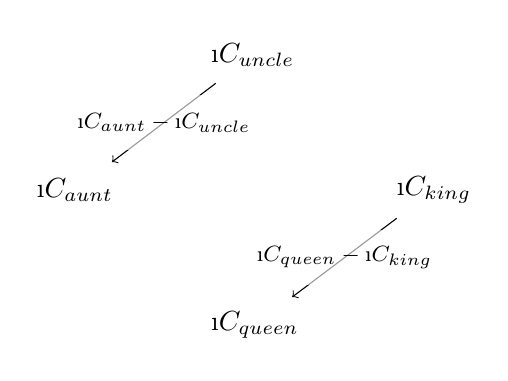
\begin{tikzpicture}
\node(a) {$\i C_{aunt}$};
\node(b)[above right = of a] {$\i C_{uncle}$};
\node(c)[below right = of a] {$\i C_{queen}$};
\node(d)[above right = of c] {$\i C_{king}$};

\draw[->] (b) -- (a) node[labe,midway]{$\i C_{aunt}-\i C_{uncle}$};
\draw[->] (d) -- (c) node[labe,midway]{$\i C_{queen}-\i C_{king}$};
\end{tikzpicture}}
}

\asidefig[\label{fig:anavecs} Vectors involved in analogy ranking tasks, this may help to understand the math in \Cref{equ:analogy}]{
	\scalebox{0.9}{\begin{tikzpicture}
	\node(a) {$\i C_a$};
	\node(b)[above right = of a] {$\i C_b$};
	\node(c)[below right = of a] {$\i C_c$};
	\node(d)[above right = of c] {$\i C_d$};
	
	\draw[->] (b) -- (a) node[labe,midway]{$\i C_a-\i C_b$};
	\draw[->] (d) -- (c) node[labe,midway]{$\i C_c- \i C_d$};
	\end{tikzpicture}}
}

One of the most notable features of  word embeddings is their ability to be used to express analogies using linear algebra.
These tasks are keyed around answering the question: \emph{b} is to \emph{a}, as what is  to \emph{c}?
For example, a semantic analogy would be answering that \natlang{Aunt} is to \natlang{Uncle} as \natlang{King} is to \natlang{Queen}.
A syntactic analogy would be answering that \natlang{King} is to \natlang{Kings} as \natlang{Queen} is to \natlang{Queens}.
The latest and largest analogy test set is presented by \tcite{gladkova2016analogy},
which evaluates embeddings on 40 subcategories of knowledge.
Analogy completion is not a practical task, but rather serves to illustrate the kinds of information being captured, and the way in which it is represented (in this case linearly).


The analogies work by relating similarities of differences between the word vectors.
When evaluating word similarity using using word embeddings a number of measures can be employed.
By far the cosine similarity is the most common.
This is given by 
\begin{equation}
\mathrm{sim}(\v u, \v v)=\frac{\v u\cdot \v v}{\left\Vert \v u\right\Vert \left\Vert \v v\right\Vert }
\end{equation}
This value becomes higher the closer the word embedding $\v u$ and $\v v$ are to each other, ignoring vector magnitude.
For word embeddings that are working well, then words with closer embeddings should have correspondingly greater similarity.
This similarity could be syntactic, semantic or other.
The analogy tasks can help identify what kinds of similarities the embeddings are capturing.

Using the similarity scores, a ranking of words to complete the analogy is found.
To find the correct word for \emph{d} in: \emph{d} is to \emph{c} as \emph{b} is to \emph{a}
the following is computed using the table of embeddings $C$ over the vocabulary $\set V$:
\begin{align}
\qquad & \argmax_{\forall d \in \set V} \mathrm{sim}(\i C_d - \i C_c, \i C_a - \i C_b)\\
\text{i.e} & \argmax_{\forall d \in \set V} \mathrm{sim}(\i C_d,\, \i C_a - \i C_b + \i C_c) \label{equ:analogy}
\end{align}
This is shown diagrammaticality in \Cref{fig:analogy,fig:anavecs}.
Sets of embeddings where the vector displacement between analogy terms are more consistent score better.


Initial results in \textcite{mikolov2013linguisticsubstructures} were relatively poor, but the surprising finding was that this worked at all.
\textcite{mikolov2013efficient} found that CBOW performed poorly for semantic tasks, but comparatively well for syntactic tasks; skip-gram performed comparatively well for both, though not quite as good in the syntactic tasks as CBOW.
Subsequent results found in  \tcite{pennington2014glove} were significantly better again for both.


\section{Co-location Factorisation}\label{sec:co-location-factorisation}

\subsection{GloVe}
\aside[Distance weighted co-occurrence and dynamic window sizing]{
	When training skip-gram and CBOW, Mikolov et al. used dynamic window sizing.
	This meant that if the specified window size was $n$, in any given training case being considered the actual window size was determined as a random number between $0$ and $n$.
	
	Pennington et al. achieve a similar effect by weighting co-occurrences within a window with inverse proportion to the distance between the word. That is to say if $\n w_i$ and $\n w_j$ occur in the same window (i.e. $|i-j|{<}n$), then rather than contributing 1 to the entry in the co-occurrence count $X_{\n w_i, \n w_j}$, they contribute $\dfrac{1}{|i-j|}$.
}


\aside[Subsampling, and weight saturation]{
	Skip-gram and CBOW models use a method called subsampling to decrease the effect of common words.
	The subsampling method is to randomly discard words from training windows based on their unigram frequency.
	This is closely related to the saturation of the co-occurrence weights as calculated by $f(X)$ used by GloVe.
	Averaged over all training cases the effect is nearly the same.
}

\aside[Key Factors Mentioned as Asides]{
	There is an interesting pattern of factors being considered as not part of the core algorithm.
	We have continued this in the side-notes of this section; with the preceding notes on Distance weighting and subsampling.	
	While the original papers consider these as unimportant to the main thrust of the algorithms \textcite{levy2015lsaisbasicallyskipgramswithexperimentstoprove} found them to be crucial hyper-parameters.
}

Skip-gram, like all probabilistic language models, is a intrinsically prediction-based method.
It is effectively optimising a neutral network to predict which words will co-occur in the with in the range of given by the context window width.
That optimisation is carried out per-context window, that is to say the network is updated based on the local co-occurrences.
In \tcite{pennington2014glove} the authors show that if one were to change that optimisation to be global over all co-occurrences,
then the optimisation criteria becomes minimising the cross-entropy between the true co-occurrence probabilities, and the value of the embedding product,
with the cross entropy measure being weighted by the frequency of the occurrence of the word.
That is to say if skip-gram were optimised globally it would be equivalent to minimising:
\begin{equation}
Loss = - \sum_{\forall \n w_i \in \set V} \sum_{\forall \n w_j  \in \set V } X_{\n w_i,\n w_j} P(\n w_j\mid \n w_i) \log (\i V_{\n w_j,:}\,\i C_{\n w_i})
\end{equation}
for $\set V$ being the vocabulary and for $X$ being the a matrix of the true co-occurrence counts, (such that $X_{\n w_i,\n w_j}$ is the number of times words $\n w_i$ and $\n w_j$ co-occur),
and for $P$ being the predicted probability output by the skip-gram.


Minimising this cross-entropy efficiently means  factorising the true co-occurrence matrix $X$,
into the input and output embedding matrices $C$ and $V$, under a particular set of weightings given by the cross entropy measure.

\textcite{pennington2014glove} propose an approach based on this idea.
For each word co-occurrence of $\n w_i$ and $\n w_j$ in the vocabulary: they attempt to find optimal values for 
the embedding tables $C$, $V$ and the per word biases $\v b$, $\v k$
such that the  function $s(\n w_i, \n w_j)$ (below) expresses an approximate log-likelihood of $\n w_i$ and $\n w_j$.
\begin{align}
\text{optimise} \quad & s(\n w_i, \n w_j) &&= \i V_{\n w_j,:}\,\i C_{\n w_i} + \iv b_{\n w_i} + \iv k_{\n w_j} \\
\text{such that} \quad & s(\n w_i, \n w_j) &&\approx \log(\i X_{\n w_i, \n w_j})
\end{align}

This is done via the minimisation of 
\begin{equation}
Loss = - \sum_{\forall \n w_i}  \sum_{\forall \n w_j} f(\i X_{\n w_i, \n w_j}) \left(s(\n w_i, \n w_j) -\log (\i X_{\n w_i, \n w_j})\right)
\end{equation}
Where $f(x)$ is a weighing between 0 and 1 given by:
\begin{equation}
f(x)=\begin{cases}
\left(\frac{x}{100}\right)^{0.75} & x<100\\
1 & \text{otherwise}
\end{cases}
\end{equation}
This can be considered as a saturating variant of the effective weighing of skip-gram being $\i X_{\n w_i, \n w_j}$.


While GloVe out-performed  skip-gram in initial tests subsequent more extensive testing in \tcite{levy2015lsaisbasicallyskipgramswithexperimentstoprove} with more tuned parameters,
found that skip-gram marginally out-performed GloVe on all tasks.




\aside[Implementing GloVe]{To implement GloVe in any technical programming language with good support for optimisation is quiet easy, as it is formed into a pure optimization problem.
It is also easy to do in a neural network framework, as these always include an optimiser.
Though unlike in normal neural network training there are no discrete training cases, just the global co-occurrence statistics.
}

\subsection{Further equivalence of  Co-location Prediction to Factorisation}

GloVe highlights the relationship between the co-located word prediction neural network models,
and the more traditional non-negative matrix factorization of co-location counts used in topic modeling.
Very similar properties were also explored for skip-grams with negative sampling in \tcite{levy2014neural} and in \tcite{li2015wordemedingasEMF} with more direct mathematical equivalence to weighed co-occurrence matrix factorisation;
Later,  \tcite{cotterell2017SkipgramisEPCA} showed the equivalence to exponential principal component analysis (PCA).
\tcite{wordvecispca} goes on to extend this to show that it is a weighted logistic PCA, which is a special case of the exponential PCA.
Many works exist in this area now.


\subsection{Conclusion}
We have now concluded that neural predictive co-location models are functionally very similar to matrix factorisation of co-location counts with suitable weightings, and suitable similarity metrics.
One might now suggest a variety of word embeddings to be created from a variety of different matrix factorisations with different weightings and constraints.
Traditionally large matrix factorisations have significant problems in terms of computational time and memory usage.
A common solution to this, in applied mathematics, is to handle the factorisation using an iterative optimisation procedure.
Training a neural network, such as skip-gram, is indeed just such an iterative optimisation procedure.




\section{Hierarchical Softmax and Negative Sampling}\label{sec:hierachical-softmax-and-negative-sampling}
Hierarchical softmax, and negative sampling are effectively alternative output layers which are computationally cheaper to evaluate than regular softmax.
They are powerful methods which pragmatically allow for large speed-up in any task which involves outputting very large classification probabilities -- such as language modelling.


\subsection{Hierarchical Softmax}\label{sec:hierarchical-softmax}
Hierarchical softmax was first presented in  \tcite{morin2005hierarchical}.
Its recent use was popularised by \tcite{mikolov2013efficient}, where words are placed as leaves in a Huffman tree, with their depth determined by their frequency.


\aside[SemHuff]{It can be noted that the Huffman encoding scheme specifies only the depth of a given word in the tree. It does not specify the order.
	\textcite{SemHuff} make use of the BlossomV algorithm \parencite{Kolmogorov2009} to pair the nodes on each layer according to their similarity.
	They found that on the language modelling task this improved performance, in the way one would expect.
	They used a lexical resource to determine similarity, however noted that a prior trained word-embedding model could be used to define similarity instead -- the new encoding can then be used to define a new model which will find new (hopefully better) embeddings.
	This is similar to the original method used by \parencite{morin2005hierarchical},
	but only using the similarity measure for reordering nodes at the same depth, after the depth is decided by Huffman encoding.
	In our own experimentation, when applying it to other tasks, we did not see large improvements.
	It is nevertheless a very interesting idea,
	and quite fun to implement and observe the results.
}

One of the most expensive parts of training and using a neural language model is  to calculate the final softmax layer output.
This is because the softmax denominator includes terms for each word in the vocabulary.
Even if only one word's probability is to be calculated, one denominator term per word in the vocabulary must be evaluated.
In hierarchical softmax, each word (output choice), is considered as a leaf on a binary tree.
Each level of the tree roughly halves the space of the output words to be considered.
The final level to be evaluated for a given word contains the word's leaf-node and another branch, which may be a leaf-node for another word, or a deeper sub-tree

The tree is normally a Huffman tree \pcite{huffman1952method}, as was found to be effective by \textcite{mikolov2013efficient}.
This means that for each word $\n w_i$, the word's depth (i.e its code's length) $l(\n w_i)$ is such that over all words:
 $\sum_{\forall \n w_j \in \set{V}} P(\n w_j)\times l(\n w_j)$ is minimised.
Where $P(\n w_i)$ is word $\n w_i$'s unigram probability, and $\set{V}$ is the vocabulary.
The approximate solution to this is that $l(\n w_i) \approx -\log_2(P(\n w_i))$.
From the tree, each word can be assign a code in the usual way, with 0 for example representing taking one branch, and 1 representing the other.
Each point in the code corresponds to a node in the binary tree, which has decision tied to it.
This code is used to transform the large  multinomial softmax classification into a series of binary logistic classifications.
It is important to understand that the layers in the tree are not layers of the neural network in the normal sense -- the layers of the tree do not have an output that is used as the input to another.
The layers of the tree are rather subsets of the neurons on the output layer, with a relationship imparted on them.

It was noted by \textcite{mikolov2013efficient}, that for vocabulary $\set{V}$:
\begin{itemize}
	\item Using normal softmax would require each evaluation to perform $|\set{V}|$ operations.
	\item Using hierarchical softmax with a balanced tree, would mean the expected number of operations across all words would be $\log_2(|\set{V}|)$.
	\item Using a Huffman tree gives the expected number of operations $\sum_{\forall \n w_j \in \set{V}} -P(\n w_j)\log_2(P(\n w_i)) = H(\set{V})$, where $H(\set{V})$ is the unigram entropy of words in the training corpus.
\end{itemize}
The worse case value for the entropy is $\log_2(|\set{V}|)$.
In-fact Huffman encoding is provably optimal in this way.
As such this is the minimal number of operations required in the average case.


\subsubsection{An incredibly gentle introduction to hierarchical softmax}
In this section, for brevity, we will ignore the bias component of each decision at each node.
It can either be handled nearly identically to the weight;
or the matrix can be written in \emph{design matrix form} with an implicitly appended column of ones;
or it can even be ignored in the implementation (as was done in \textcite{mikolov2013efficient}).
The reasoning for being able to ignore it is that the bias in normal softmax encodes unigram probability information;
in hierarchical softmax, when used with the common Huffman encoding, its the tree's depth in tree encodes its unigram probability. In this case, not using a bias would at most cause an error proportionate to $2^{-k}$, where $k$ is the smallest integer such that $2^{-k}>P(\n w_i)$.



\paragraph{First consider a binary tree with just 1 layer and 2 leaves}
The leaves are $\n n_{00}$ and $\n n_{01}$, each of these leaf nodes corresponds to a word from the vocabulary, which has size two, for this toy example.

\asidefig[Tree for 2 words]{\begin{tikzpicture}
	\Tree [.$\n n_0$ 
		$\n n_{00}$
		$\n n_{01}$ ]
\end{tikzpicture}}
	
From the initial root which we call $\n n_{0}$, we can go to
either node $\n n_{00}$ or node $\n n_{01}$, based on the input from the
layer below which we will call $\v z$.


Here we write $\n n_{01}$ to represent the event of the first non-root
node being the branch given by following left branch, while $\n n_{01}$
being to follow the right branch.
(The order within the same level is arbitrary in any-case, but for our visualisation purposes we'll used this convention.) 

We are naming the root node as a notation convenience so we can talk
about the decision made at $\n n_{0}$. 
Note that $P(\n n_{0})=1$, as all words include the root-node on their path.

We wish to know the probability of the next node being the left node (i.e.
$P(\n n_{00}\mid \v z)$ ) or the right-node (i.e. $P(\n n_{01}\mid \v z)$).
As these are leaf nodes, the prediction either equivalent to the prediction of one or the other of the two words in our vocabulary.

We could represent the decision with a softmax with two outputs.
However, since it is a binary decision, we do not need a softmax, we
can just use a sigmoid.
\begin{equation}
P(\n n_{01}\mid \v z)= 1 - P(\n n_{00}\mid \v z)
\end{equation}

The weight matrix for a sigmoid layer has a number of columns governed
by the number of outputs.
As there is only one output, it is just a row vector.
We are going to index it out of a matrix $V$.
For the notation, we will use index $0$ as it is associated with the decision at node $\n n_{0}$.
Thus we call it $\i V_{0,:}$.

\aside[$\i V_{0,:} \v z$ is a dot product]{We mentioned in the marginalia earlier, but just as an extra reminder: the matrix product of a row vector like $\i V_{0,:}$  with a (column) vector like $\v z$ is their vector dot product.}

\begin{align}
P(\n n_{00} \mid \v z) &=\sigma(\i V_{0,:} \v z) \\
P(\n n_{01} \mid \v z) &=1-\sigma(\i V_{0,:} \v z)
\end{align}
Note that for the sigmoid function: $1-\sigma(x)=\sigma(-x)$.
Allowing the formulation to be written:
\begin{equation}
P(\n n_{01}\mid \v z)=\sigma({-}\i V_{0,:}\v z)
\end{equation}
thus
\begin{equation}
P(\n n_{0i}\mid \v z)=\sigma(({-}1)^i \i V_{0,:}\v z) \label{equ:hsoftmaxbinfirst}
\end{equation}
Noting that in \Cref{equ:hsoftmaxbinfirst}, $i$ is either 0 (with ${-1}^0=1$) or 1 (with ${-1}^1={-}1$)).


\paragraph{Now consider 2 layers with 3 leaves}

Consider a tree with nodes: $\n n_{0}$, $\n n_{00}$,$\n n_{000}$, $\n n_{001}$, $\n n_{01}$.
The leaves are $\n n_{000}$, $\n n_{001}$, and $\n n_{01}$, each of which represents one of the 3 words from the vocabulary.

\asidefig[Tree for 3 words]{\begin{tikzpicture}
	\Tree [ .$\n n_0$ 
	[ .$\n n_{00}$
	$\n n_{000}$
	$\n n_{001}$ ]
	$\n n_{01}$ ]
	\end{tikzpicture}}

From earlier we still have:

\begin{align}
P(\n n_{00}\mid \v z)&=\sigma(\i V_{0,:}\v z)\\
P(\n n_{01}\mid \v z)&=\sigma(-\i V_{0,:}\v z)
\end{align}
We must now to calculate $P(\n n_{000}\mid \v z)$.
Another  binary decision must be made at node $\n n_{00}$.
The decision at $\n n_{00}$ is to find out if the predicted next node is $\n n_{000}$ or $\n n_{001}$.
This decision is made, with the assumption that we have reached $\n n_{00}$ already.

So the decision is defined by $P(\n n_{000}\mid z,\:\n n_{00})$
is given by:
\begin{align}
P(\n n_{000}\mid \v z)&=P(\n n_{000}\mid \v z,\:\n n_{00})\,P(\n n_{00}\mid \v z) \\
P(\n n_{000}\mid \v z,\n n_{00})&=\sigma(\i V_{00,:}\v z) \\
P(\n n_{001}\mid \v z,\n n_{00})&=\sigma(-\i V_{00,:}\v z)
\end{align}

We can use the conditional probability chain rule to recombine
to compute the three leaf nodes final probabilities.
\begin{align}
P(\n n_{01}\mid \v z)&=\sigma(-\i V_{0,:}\v z) \\
P(\n n_{000}\mid \v z)&=\sigma(\i V_{00,:}\v z)\sigma(\i V_{0,:}\v z) \\
P(\n n_{001}\mid \v z)&=\sigma(-\i V_{00,:}\v z)\sigma(\i V_{0,:} \v z)
\end{align}

\paragraph{Continuing this logic}

Using this system,
we know that for a node encoded at position $[0\n t_{1}\n t_{2}\n t_{3}\ldots\n t_{L}]$
, e.g. $[010\ldots1]$,
its probability can be found recursively as: 
\begin{multline}
P(\n n_{0\n t_{1}\ldots\n t_{L}}\mid \v z) =\\
\quad P(\n n_{0\n t_{1}\ldots\n t_{L}}\mid \v z,\,\n n_{0\n t_{1}\ldots\n t_{L-1}})\,P(\n n_{0\n t_{1}\ldots\n t_{L-1}}\mid \v z)
\end{multline}
Thus:
\begin{align}
%
P(\n n_{0\n t_{1}}\mid \v z)&=\sigma\left((-1)^{\n t_{1}}\i V_{0,:} \v z\right)\\
%
P(\n n_{0\n t_{1},\n t_{2}}\mid \v z,\,\n n_{0\n t_{1}})&=\sigma\left((-1)^{\n t_{2}} \i V_{0\n t_{1}, :} \v z\right)\\
%
P(\n n_{0\n t_{1}\ldots\n t_{i}}\mid \v z,\,\n n_{0\n t_{1}\ldots\n t_{i-1}})&=\sigma\left((-1)^{\n t_{i}} \i V_{0\n t_{1}\ldots\n t_{i-1}, :} \v z\right)
\end{align}

The conditional probability chain rule, is applied to get:
\begin{equation}
P(\n n_{0\n t_{1}\ldots\n t_{L}}\mid \v z)=\prod_{i=1}^{i=L}\sigma\left((-1)^{\n t_{i}} \i V_{0\n t_{1}\ldots\n t_{i-1},:} \v z\right)
\end{equation}

\subsubsection{Formulation}

\aside[Combining multiplications]{
	If one wants to find both $\i V_{00,:} \v z$ and $\i V_{0,:} \v z$,
	then this can be done using matrices simultaneously, thus potentially taking advantage
	of optimized matrix multiplication routines.
	
	$\left[\begin{array}{c}
	\i V_{0,:}\\
	\i V_{00,:}
	\end{array}\right]z=\left[\begin{array}{c}
	\i V_{0,:} \v z\\
	\i V_{00,:} \v z
	\end{array}\right]$
	
	Thus the whole product for all of the decisions can be written as
	$V \v z$.
	The problem then becomes indexing the relevant node rows.
	
	However computing  every single decision is beyond what is required for most uses: hierarchical softmax lets us only compute the decisions that are on the path to the word-leaf we which we wish to query.
	Computing all of them is beyond what is required.
	
	Packing tree node elements into a matrix with fast indexing is a non-trivial problem.
	The details on optimising such multiplications and tree packing are beyond the scope of this book.
	
	In general there may be very little scope here for optimisation,
	as on most hardware (and BLAS systems) matrix products with $n$ columns, takes a similar amount of time to $n$ vector dot products.
	As such storing the row vectors of $V$ in a hashmap indexed by node-path, and looping over them as required may be more practical.
	
	In languages/libraries with slow looping constructs (numpy, R, octave), where calling into suitable library routines is much faster, this may give some speed-up;
	but even here it is likely to be minor.
	The time may be better spent writing a C extension library to do this part of the program.
	Or learning to use a language with fast for loops (e.g. Julia \parencite{Julia}).
}

The formulation above is not the same as in other works.
This subsection shows the final steps to reach the conventional form used in \textcite{mikolovSkip}.


Here  we have determined that the 0th/left branch represents the positive choice, and the other probability is defined in terms of this.
It is equivalent to have the 1th/right branch representing the positive choice:
\begin{equation}
P(\n n_{0\n t_{1}\ldots\n t_{L}}\mid \v z)=\prod_{i=1}^{i=L}\sigma\left((-1)^{\n t_{i}+1} \i V_{0\n t_{1}\ldots\n t_{i-1}, :} \v z\right)
\end{equation}


or to allow it to vary per node: as in the formulation of \tcite{mikolovSkip}.
In that work they use $ch(n)$ to represent an arbitrary child node of the node $n$
and use an indicator function $\left\llbracket a=b\right\rrbracket =\begin{cases}
1 & a=b\\
-1 & a\ne b
\end{cases}$ such that they can write $\left\llbracket \n n_b =ch(\n n_a)\right\rrbracket$ which will be 1 if $\n n_a$ is an arbitrary (but consistent) child of $\n n_b$, and 0 otherwise.

\aside[How does this relate to word vectors?]{
After the length of this section, one may have forgotten why we are doing this in the first place.
Recall that CBOW, skip-gram and all other language modelling based word embedding methods are based around predicting
 $P(\n w_o \mid \n w_i,\ldots, \n w_{j})$ for some words.
For skip-gram that is just $P(\n w_o\mid \n w_i)$.
The term $\n n_{0\n t_{1}\ldots\n t_{L}}$ 
in  $P(\n n_{0\n t_{1}\ldots\n t_{L}}\mid z)$, 
just represents as a path through the tree to the leaf node which represents the word 
$\n w_o$. i.e $P(\n n_{0\n t_{1}\ldots\n t_{L}}\mid z)=P(\n w_o\mid z)$.
The output of the final hidden layer is $z$  (i.e. the $z$ is the input to the output layer)
In normal language models $z$ encodes all the information about what the model knows of predictions based on $\n w_i\ldots,\n w_{j}$. $z$ is thus a proxy term in the conditional probability for those words.
In skip-gram there is no hidden layer, and it is just $z = \i C_{\n w_i}$ proxying only for $w_i$,
and the model defines its probability output by $P(\n w_o\mid \n w_i) = P(\n w_o\mid \i C_{\n w_i})$.
}


\begin{multline}
P(\n n_{0\n t_{1}\ldots\n t_{L}}\mid \v z)=\\
\prod_{i=1}^{i=L} \sigma\left(
	\left\llbracket 
		\n n_{0\n t_{1}\ldots\n t_{i}}
		=ch(\n n_{0\n t_{1}\ldots\n t_{i-1}})
	\right\rrbracket
	\i V_{0\n t_{1}\ldots\n t_{i-1},:}
	\v z
\right)
\end{multline}


There is no functional difference between the three formulations.
Though the final one is perhaps a key reason for the difficulties in understanding the hierarchical softmax algorithm.

\subsubsection{Loss Function}\label{sec:softmax-loss-function}
\aside[The gradient calculations]{They are not fun. They never are for back-propagation. We recommend using a framework with automated differentiation, and/or performing gradient checks against a numerical differentiation tool (simple finite-differencing will do in a pinch).}

Using normal softmax, during the training, the cross-entropy between the model's predictions and the ground truth as given in the training set is minimised.
Cross entropy is given by

\begin{equation}
CE(P^\star, P) = \sum_{\forall \n w_i\in \set{V}} \sum_{\forall \n z_j \in \set{Z}} -P^\star(\n w_i \mid \n z_j) \log P(\n w_i \mid \n z_j)
\end{equation}
Where $P^\star$ is the true distribution, and $P$ is the approximate distribution given by our model (in other sections we have abused notation to use $P$ for both).
$\set Z$ is the set of values that are input into the model, (or equivalently the values derived from them from lower layers) -- Ithe context words in language modelling.
$\set V$ is the set of outputs, the vocabulary in language modeling.
The training dataset $\seq X$ consists of pairs from $\set V \times \set Z$.

The true probabilities (from $P^\star$) are implicitly given by the frequency of the training pairs in the training dataset $\seq X$.
\begin{equation}
Loss=CE(P^\star, P) = \frac{1}{|\seq{X}|} \sum_{\mathrlap{\!\!\!\!\!\forall (\n w_i, \n z_i) \in \seq{X}}} -\log P(\n w_i \mid \n z_i)
\end{equation}


The intuitive understanding of this, is that we are maximising the probability estimate of all pairings which actually occur in the training set, proportionate to how often the occur.
Note that the $\set Z$ can be non-discrete values, as was the whole benefit of using embeddings, as discussed in \Cref{sec:the-neural-probabilistic-language-model}.

This works identically for hierarchical softmax as for normal softmax.
It is simply a matter of substituting in the (different) equations for $P$.
Then applying back-propagation as usual.

\subsection{Negative Sampling}\label{sec:negative-sampling}

%\pdfcomment{This section is currently written using skip-gram no hidden layer, so uses $\n w_i$, but it doesn't have to. It could be rewritten like the previous, to use $z$ for the output of the pre-output layer. Which might just so happen to bt $\n w_i$ in the case of the skip-gram. }

Negative sampling was introduced in \tcite{mikolovSkip} as another method to speed up this problem.
Much like hierarchical softmax in its purpose.
However, negative sampling does not modify the network's output, but rather the loss function.


Negative Sampling is a simplification of Noise Contrast Estimation \pcite{gutmann2012noise}.
Unlike Noise Contrast Estimation (and unlike softmax), it does not in fact result in the model converging to the same output as if it were trained with softmax and cross-entropy loss.
However the goal with these word embeddings is not to actually perform the language modelling task, but only to capture a high-quality vector representation of the words involved.

\subsubsection{A Motivation of Negative Sampling}
Recall from \Cref{sec:skip-gram} that the (supposed) goal, is to estimate $P(\n w_j\mid \n w_i)$.
In truth, the goal is just to get a good representation, but that is achieved via optimising the model to predict the words.
In  \Cref{sec:skip-gram}  we considered the representation of $P(\n w_j\mid \n w_i)$ as the $\n w_j$th element of the softmax output.

\begin{align}
P(\n w_j \mid \n w_i) & = \i {\softmax(V\,\i C_{\n w_i})}_{\n w_j} \\
P(\n w_j \mid \n w_i) & = \frac{\exp{\i V_{\n w_j,:} \i C_{\n w_i}}}{\sum_{k=1}^{k=N} \exp{\i V_{k,:} \i C_{k}}}
\end{align}

\aside[Why is not using softmax wrong?]{The notation abuse may be hiding just how bad it is to not use softmax.
Recall that the true meaning of %\\
\mbox{$P(\n w_j \mid \n w_i)$} is actually  %\\
\mbox{$P(\n W_j{=}\n w_j \mid \n W_i{=}\n w_i)$}.
By not using softmax, with its normalising denominator this means that:
\mbox{$\sum_{\forall \n w_j \in \set{V}} P(\n w_j \mid \n w_i) \neq 1$} \\(except by coincidence).
}


This is not the only valid representation.
One could use a sigmoid neuron for a direct answer to the co-location probability of $\n w_j$ occurring near $\n w_i$.
Though this would throw away the promise of the probability distribution to sum to one across all possible words that could be co-located with $\n w_i$.
That promise could be enforced by other constraints during training, but in this case it will not be.
It is a valid probability if one does not consider it as a single categorical prediction, but rather as independent predictions.

\begin{align}
&P(\n w_j \mid \n w_i) & = \i \sigma(V\,\i C_{\n w_i})_{\n w_j} \\
\text{i.e.}\quad&P(\n w_j \mid \n w_i) & = \i \sigma(\i V_{\n w_j,:} \i C_{\n w_i})
\end{align}


Lets start from the cross-entropy loss.%
\aside[Loss Function]{Readers may want to reread \Cref{sec:softmax-loss-function} to brush up on how we use the training dataset as a ground truth probability estimate implicitly when using cross-entropy loss. When doing so one should remember that that the conditioning term, $z$, for skip-grams is the co-located words as there is no hidden layer.}
%
In training word $\n w_j$ does occur near $\n w_i$, we know this because they are a training pair presented from the training dataset $\seq{X}$.
Therefore, since it occurs, we could make a loss function based on minimising the negative log-likelihood of all observations.
\begin{equation}
Loss = \sum_{\mathclap{\forall (\n w_i,\n w_j)\in \seq{X}}} -\log P(\n w_j\mid \n w_i)
\end{equation}
This is the cross-entropy loss, excluding the scaling factor for how often it occurs.

However, we are not using softmax in the model output,
which means that there is no trade off for increasing (for example) $P(\n w_1\mid \n w_i)$ vs $P(\n w_2\mid \n w_i)$.
This thus admits the trivially optimal solution $\forall \n w_j\in \set{V}$ $P(\n w_j \mid \n w_i) = 1$.
This is obviously wrong -- even beyond not being a proper distribution -- some words are more commonly co-occurring than others.

So from this we can improve the statement.
What is desired from the loss function is to reward models that predict  the probability of words that \emph{do} co-occur as being higher, than the probability of words that \emph{do not}.
We know that $\n w_j$ does occur near $\n w_i$ as it is in the training set.
Now, let us select via some arbitrary means a $\n w_k$ that does not -- a negative sample.
We want the loss function to be such that $P(\n w_k\mid \n w_i) < P(\n w_j\mid \n w_i)$.
So for this single term in the loss we would have:
\begin{equation}
loss(\n w_j,\n w_i) =  \log P(\n w_k\mid \n w_i) - \log P(\n w_j\mid \n w_i)
\end{equation}
\aside[Most words do not co-occur]{
	Some simple reasoning can account for this as a reasonable consequence of Zipf's law \parencite{zipf1949human} and a prior of the principle of indifference, but there is a further depth to it as explained by \textcite{ha2009extending}.}%
%
%
The question is then: how is the negative sample $\n w_k$ to be found?
One option would be to deterministically search the corpus for these negative samples, making sure to never select words that actually do co-occur.
However that would require enumerating the entire corpus.
We can instead just pick them randomly, we can sample from the unigram distribution.
As statistically, in any given corpus most words do not co-occur, 
a randomly selected word in all likelihood will not be one that truly does co-occur
-- and if it is, then that small mistake will vanish as noise in the training,
overcome by all the correct truly negative samples.

\aside[Is \Cref{equ:samplesloss} a function?]{No, at the point at which the Loss started including randomly selected samples, it ceased to be a function in the usual mathematical sense. It is still a function in the common computer programming sense though -- it is just not deterministic.}

At this point, we can question, why limit ourselves to one negative sample?
We could take many, and do several at a time,
and get more confidence that $P(\n w_j\mid \n w_i)$ is indeed greater than other (non-existent) co-occurrence probabilities.
This gives the improved loss function of 

\begin{equation}
loss(\n w_j,\n w_i) = 
\left(\sum_{\mathrlap{\!\!\!\!\!\!\forall \n w_k \in \mathrm{samples}(\d D_{1g})}}
\log P(\n w_k\mid \n w_i) \right)
- \log P(\n w_j\mid \n w_i)
\label{equ:samplesloss}
\end{equation}
where $\d D_{1g}$ stands for the unigram distribution of the vocabulary
and $\mathrm{samples}(\d D_{1g})$ is a function that returns some number of samples from it.

Consider, though is this fair to the samples?
We are taking them as representatives of all words that do not co-occur.
Should a word that is unlikely to occur at all, \emph{but was unlucky enough to be sampled}, contribute the same to the loss as a word that was very likely to occur?
More reasonable is that the loss contribution should be in proportion to how likely the samples were to occur.
Otherwise it will add unexpected changes and result in noisy training.
Adding a weighting based on the unigram probability ($\d P_{1g}(\n w_k)$) gives:
%
\begin{multline}
loss(\n w_j,\n w_i) = \\
\left(\sum_{\mathrlap{\!\!\!\!\!\!\forall \n w_k \in \text{samples}(\d D_{1g})}}
\d P_{1g}(\n w_k) \log P(\n w_k\mid \n w_i) \right)
-\log P(\n w_j\mid \n w_i)
\end{multline}


The expected value is defined by
\begin{equation}
\expected_{X \sim D} \left[ f(x) \right]= \sum_{\text{$\forall x$ values for $X$}} \d P_d f(x)
\end{equation}

In an abuse of notation, we apply this to the samples, as a sample expected value and write:
\begin{equation}
	\sum_{k=1}^{k=n} \expected_{\n w_k \sim \d D_{1g}} [\log P(\n w_k\mid \n w_i)]
\end{equation}
to be the sum of the $n$ samples expected values.
This notation (abuse) is as used in \tcite{mikolovSkip}.
It gives the form:
\begin{multline}
loss(\n w_j,\n w_i) = \\
\left(\sum_{k=1}^{k=n} \expected_{\n w_k \sim \d D_{1g}} [\log P(\n w_k\mid \n w_i)]) \right)
-\log P(\n w_j\mid \n w_i)
\end{multline}

Consider that the choice of unigram distribution for the negative samples is not the only choice.
For example, we might wish to increase the relative occurrence of rare words in the negative samples, to help them fit better from limited training data.
This is commonly done via subsampling in the positive samples (i.e. the training cases)).
So we replace $\d D_{1g}$ with $\d D_{ns}$ being the distribution of negative samples from the vocabulary,
to be specified as a hyper-parameter of training.

\textcite{mikolovSkip} uses a distribution such that 
\begin{equation}
\d P_{\d D_{ns}}(\n w_k) =  \frac{\d P_{\d D_{1g}}(\n w_k)^{\frac{2}{3}}}{\sum_{\forall \n w_o\in \set{V}} \d P_{\d D_{1g}}(\n w_o)^{\frac{2}{3}}}
\end{equation}
which they find to give better performance than the unigram or uniform distributions.

Using this, and substituting in the sigmoid for the probabilities, this becomes:
\begin{multline}
loss(\n w_j,\n w_i) = \\
\left(\sum_{k=1}^{k=n} \expected_{\n w_k \sim \d D_{ns}} [\log \sigma(\i V_{\n w_k,:}\i C_{\n w_i}) \right)
-\log \sigma(\i V_{\n w_j,:} \i C_{\n w_i})
\end{multline}

By adding a constant we do not change the optimal value.
If we add the constant $-K$, we can subtract 1 in each sample term.

\begin{multline}
loss(\n w_j,\n w_i) = \\
\left(\sum_{k=1}^{k=n} \expected_{\n w_k \sim \d D_{ns}} [-1 + \log \sigma(\i V_{\n w_k,:} \i C_{\n w_i}) \right)
-\log \sigma(\i V_{\n w_j,:}\i C_{\n w_i})
\end{multline}

Finally we make use of the identity $1-\sigma(\v z) = \sigma(-\v z)$ giving:
\begin{multline}
loss(\n w_j,\n w_i) = \\
-\log \sigma(\i V_{\n w_j,:} \i C_{\n w_i}) 
- \sum_{k=1}^{k=n} \expected_{\n w_k \sim \d D_{ns}} [\log \sigma(- \i V_{\n w_k,:} \i C_{\n w_i})] 
\end{multline}

Calculating the total loss over the training set $\seq{X}$:
\begin{multline}
Loss = \quad -\sum_{\mathclap{\forall (\n w_i,\n w_j)\in \seq{X}}}\\
\left(
\log \sigma(\i V_{\n w_j,:} \i C_{\n w_i}) 
+ \sum_{k=1}^{k=n} \expected_{\n w_k \sim \d D_{ns}} [\log \sigma(- \i V_{\n w_k,:} \i C_{\n w_i})] 
\right)
\end{multline}

This is the negative sampling loss function used in  \textcite{mikolovSkip}.
Perhaps the most confusing part of this is the notation.
Without the abuses around expected value, this is written:
\begin{multline}
Loss = \quad -\sum_{\mathclap{\forall (\n w_i,\n w_j)\in \seq{X}}}\\
\biggl( \log \sigma(\i V_{\n w_j,:} \i C_{\n w_i}) 
+ \sum_{\mathclap{\forall \n w_k \in \text{samples}(\d D_{ns})}}
\d P_{\d D_{ns}}(\n w_k) \log \sigma(- \i V_{\n w_k,:} \i C_{\n w_i})
\biggr)
\end{multline}



\section{Natural Language Applications -- beyond language modeling}
While statistical language models are useful, they are of-course in no way the be-all and end-all of natural language processing.
Simultaneously with the developments around representations for the language modelling tasks, work was being done on solving other NLP problems using similar techniques \pcite{collobert2008unified}.


\subsection{Using Word Embeddings as Features}

\aside[Pretrained \\ Word-Embeddings]{
	Pretrained Word Embeddings are available for most models discussed here.
	They are trained on a lot more data than most people have reasonable access to.
	It can be useful to substitute word embeddings as a representation in most systems,
	or to use them as initial value for neural network systems that will learn them as they train the system as a whole.
	There are many many online pretrained word embeddings.
	One of the more recent and comprehensive set is that of \tcite{bojanowski2016enriching} (based on a skip-gram extension),
	\url{https://fasttext.cc/docs/en/pretrained-vectors.html} They provide embeddings for 294 languages, trained on Wikipedia based on the work of  which is an extension to skip-grams.
}

\tcite{turian2010word} discuss what is now perhaps the most important use of word embeddings.
The use of the embeddings as features, in unrelated feature driven models.
One can find word embeddings using any of the methods discussed above.
These embeddings can be then used as features instead of, for example bag of words or hand-crafted feature sets.
\textcite{turian2010word} found improvements on the state of the art for chunking and Named Entity Recognition (NER), using the word embedding methods of that time.
Since then, these results have been superseded again using newer methods.


\section{Aligning Vector Spaces Across Languages}\label{sec:aligning-vector-spaces-across-languages}
Given two vocabulary vector spaces, for example one for German and one for English,
a natural and common question is if they can be aligned such that one has a single vector space for both.
Using canonical correlation analysis (CCA) one can do exactly that.
There also exists generalised CCA for any number of vector spaces \pcite{gcca},
as well as kernel CCA for a non-linear alignment.

The inputs to CCA, are two sets of vectors, normally expressed as matrices.
We will call these:
$C \in \mathbb{R}^{\d n_C \times \d m_C}$ and $V \in \mathbb{R}^{\d n_V \times \d m_V}$.
They are both sets of vector representations, not necessarily of the same dimensionality.
They could be the output of any of the embedding models discussed earlier,
or even a sparse (non-embedding) representations such as the point-wise mutual information of the co-occurrence counts.
The other input is series  pairs of elements from within those those sets that are to be aligned.
We will call the elements from that series of pairs from the original sets $\d C_\star$ and $\d V_\star$ respectively.
$\d C_\star$  and $\d V_\star$ are subsets of the original sets, with the same number of representations.
In the example of applying this to translation, if each vector was a word embedding:
$\d C_\star$  and $\d V_\star$ would contains only words with a single known best translation, and this does not have to be the whole vocabulary of either language.


%
By performing CCA one solves to find a series of vectors (also expressed as a matrix), $S=\left[ \dv s_1 \ldots \dv s_d \right]$ and $T= \left[ \dv t_1 \ldots \dv t_d \right]$,
such that the correlation between $\d C_\star \dv s_i$ and $\d V_\star \dv t_i$ is maximised,
with the constraint that for all $j<i$ that $\d C_\star \dv s_i$ is uncorrelated with $\d C_\star \dv s_j$  and that  $ \d V_\star \dv t_i$ is uncorrelated with $\d V_\star \dv t_j$.
This is very similar to principal component analysis (PCA), and like PCA the number of components to use ($d$) is a variable which can be decreased to achieve dimensionality reduction.
When complete, taking $S$ and $T$ as matrices gives projection matrices which project $C$ and $V$ to a space where aligned elements are as correlated as possible.
The new common vector space embeddings are given by:
$C S$ and $V T$.
Even for sparse inputs the outputs will be dense embeddings.
%\pdfcomment{Check this, both for correctness in description, and for correctness in notation. In particular recheck dimensions WRT transposing/row/column}

\textcite{faruqui2014improving} investigated this primarily as a means to use additional data to improve performance on monolingual tasks.
In this, they found a small and inconsistent improvement.
However, we suggest it is much more interesting as a multi-lingual tool.
It allows similarity measures to be made between words of different languages.
\tcite{translating-unknown-words-2016} use this as part of a hybrid system to translate out of vocabulary words.
\tcite{klein2015associating} use it to link word-embeddings with image embeddings.

\tcite{dhillon2011multi} investigated using this to create word-embeddings.
We noted in \Cref{equ:skipgram-output}, that skip-gram maximise the similarity of the output and input embeddings according to the dot-product.
CCA also maximises similarity (according the correlation), between the vectors from one set, and the vectors for another.
As such given representations for two words from the same context, initialised randomly,
CCA could be used repeatedly to optimise towards good word embedding capturing shared meaning from contexts.
This principle was used by \tcite{dhillon2011multi}, though their final process more complex than described here.
It is perhaps one of the more unusual ways to create word embeddings as compared to any of the methods discussed earlier.

Aligning embeddings using linear algebra after they are fully trained is not the only means to end up with a common vector space.
One can also directly train embeddings on multiple languages concurrently as was done in \tcite{shi2015learningbiligualcofactorisation}, amongst others.
Similarly, on the sentence embedding side \textcite{zou2013bilingual}, and \tcite{socherDTRNN} train embeddings from different languages and modalities (respectively) directly to be near to their partners (these are discussed in \Cref{sec:sentence-representations-and-beyond}).
A survey paper on such methods was recently published by \tcite{Ruder17crosslingreview}.


%\printbibliography

\end{document}
